% Options for packages loaded elsewhere
% Options for packages loaded elsewhere
\PassOptionsToPackage{unicode}{hyperref}
\PassOptionsToPackage{hyphens}{url}
\PassOptionsToPackage{dvipsnames,svgnames,x11names}{xcolor}
%
\documentclass[
  11pt,
  letterpaper,
]{article}
\usepackage{xcolor}
\usepackage[margin=1in,headheight=14pt]{geometry}
\usepackage{amsmath,amssymb}
\setcounter{secnumdepth}{-\maxdimen} % remove section numbering
\usepackage{iftex}
\ifPDFTeX
  \usepackage[T1]{fontenc}
  \usepackage[utf8]{inputenc}
  \usepackage{textcomp} % provide euro and other symbols
\else % if luatex or xetex
  \usepackage{unicode-math} % this also loads fontspec
  \defaultfontfeatures{Scale=MatchLowercase}
  \defaultfontfeatures[\rmfamily]{Ligatures=TeX,Scale=1}
\fi
\usepackage{lmodern}
\ifPDFTeX\else
  % xetex/luatex font selection
\fi
% Use upquote if available, for straight quotes in verbatim environments
\IfFileExists{upquote.sty}{\usepackage{upquote}}{}
\IfFileExists{microtype.sty}{% use microtype if available
  \usepackage[]{microtype}
  \UseMicrotypeSet[protrusion]{basicmath} % disable protrusion for tt fonts
}{}
\makeatletter
\@ifundefined{KOMAClassName}{% if non-KOMA class
  \IfFileExists{parskip.sty}{%
    \usepackage{parskip}
  }{% else
    \setlength{\parindent}{0pt}
    \setlength{\parskip}{6pt plus 2pt minus 1pt}}
}{% if KOMA class
  \KOMAoptions{parskip=half}}
\makeatother
% Make \paragraph and \subparagraph free-standing
\makeatletter
\ifx\paragraph\undefined\else
  \let\oldparagraph\paragraph
  \renewcommand{\paragraph}{
    \@ifstar
      \xxxParagraphStar
      \xxxParagraphNoStar
  }
  \newcommand{\xxxParagraphStar}[1]{\oldparagraph*{#1}\mbox{}}
  \newcommand{\xxxParagraphNoStar}[1]{\oldparagraph{#1}\mbox{}}
\fi
\ifx\subparagraph\undefined\else
  \let\oldsubparagraph\subparagraph
  \renewcommand{\subparagraph}{
    \@ifstar
      \xxxSubParagraphStar
      \xxxSubParagraphNoStar
  }
  \newcommand{\xxxSubParagraphStar}[1]{\oldsubparagraph*{#1}\mbox{}}
  \newcommand{\xxxSubParagraphNoStar}[1]{\oldsubparagraph{#1}\mbox{}}
\fi
\makeatother

\usepackage{color}
\usepackage{fancyvrb}
\newcommand{\VerbBar}{|}
\newcommand{\VERB}{\Verb[commandchars=\\\{\}]}
\DefineVerbatimEnvironment{Highlighting}{Verbatim}{commandchars=\\\{\}}
% Add ',fontsize=\small' for more characters per line
\usepackage{framed}
\definecolor{shadecolor}{RGB}{241,243,245}
\newenvironment{Shaded}{\begin{snugshade}}{\end{snugshade}}
\newcommand{\AlertTok}[1]{\textcolor[rgb]{0.68,0.00,0.00}{#1}}
\newcommand{\AnnotationTok}[1]{\textcolor[rgb]{0.37,0.37,0.37}{#1}}
\newcommand{\AttributeTok}[1]{\textcolor[rgb]{0.40,0.45,0.13}{#1}}
\newcommand{\BaseNTok}[1]{\textcolor[rgb]{0.68,0.00,0.00}{#1}}
\newcommand{\BuiltInTok}[1]{\textcolor[rgb]{0.00,0.23,0.31}{#1}}
\newcommand{\CharTok}[1]{\textcolor[rgb]{0.13,0.47,0.30}{#1}}
\newcommand{\CommentTok}[1]{\textcolor[rgb]{0.37,0.37,0.37}{#1}}
\newcommand{\CommentVarTok}[1]{\textcolor[rgb]{0.37,0.37,0.37}{\textit{#1}}}
\newcommand{\ConstantTok}[1]{\textcolor[rgb]{0.56,0.35,0.01}{#1}}
\newcommand{\ControlFlowTok}[1]{\textcolor[rgb]{0.00,0.23,0.31}{\textbf{#1}}}
\newcommand{\DataTypeTok}[1]{\textcolor[rgb]{0.68,0.00,0.00}{#1}}
\newcommand{\DecValTok}[1]{\textcolor[rgb]{0.68,0.00,0.00}{#1}}
\newcommand{\DocumentationTok}[1]{\textcolor[rgb]{0.37,0.37,0.37}{\textit{#1}}}
\newcommand{\ErrorTok}[1]{\textcolor[rgb]{0.68,0.00,0.00}{#1}}
\newcommand{\ExtensionTok}[1]{\textcolor[rgb]{0.00,0.23,0.31}{#1}}
\newcommand{\FloatTok}[1]{\textcolor[rgb]{0.68,0.00,0.00}{#1}}
\newcommand{\FunctionTok}[1]{\textcolor[rgb]{0.28,0.35,0.67}{#1}}
\newcommand{\ImportTok}[1]{\textcolor[rgb]{0.00,0.46,0.62}{#1}}
\newcommand{\InformationTok}[1]{\textcolor[rgb]{0.37,0.37,0.37}{#1}}
\newcommand{\KeywordTok}[1]{\textcolor[rgb]{0.00,0.23,0.31}{\textbf{#1}}}
\newcommand{\NormalTok}[1]{\textcolor[rgb]{0.00,0.23,0.31}{#1}}
\newcommand{\OperatorTok}[1]{\textcolor[rgb]{0.37,0.37,0.37}{#1}}
\newcommand{\OtherTok}[1]{\textcolor[rgb]{0.00,0.23,0.31}{#1}}
\newcommand{\PreprocessorTok}[1]{\textcolor[rgb]{0.68,0.00,0.00}{#1}}
\newcommand{\RegionMarkerTok}[1]{\textcolor[rgb]{0.00,0.23,0.31}{#1}}
\newcommand{\SpecialCharTok}[1]{\textcolor[rgb]{0.37,0.37,0.37}{#1}}
\newcommand{\SpecialStringTok}[1]{\textcolor[rgb]{0.13,0.47,0.30}{#1}}
\newcommand{\StringTok}[1]{\textcolor[rgb]{0.13,0.47,0.30}{#1}}
\newcommand{\VariableTok}[1]{\textcolor[rgb]{0.07,0.07,0.07}{#1}}
\newcommand{\VerbatimStringTok}[1]{\textcolor[rgb]{0.13,0.47,0.30}{#1}}
\newcommand{\WarningTok}[1]{\textcolor[rgb]{0.37,0.37,0.37}{\textit{#1}}}

\usepackage{longtable,booktabs,array}
\newcounter{none} % for unnumbered tables
\usepackage{calc} % for calculating minipage widths
% Correct order of tables after \paragraph or \subparagraph
\usepackage{etoolbox}
\makeatletter
\patchcmd\longtable{\par}{\if@noskipsec\mbox{}\fi\par}{}{}
\makeatother
% Allow footnotes in longtable head/foot
\IfFileExists{footnotehyper.sty}{\usepackage{footnotehyper}}{\usepackage{footnote}}
\makesavenoteenv{longtable}
\usepackage{graphicx}
\makeatletter
\newsavebox\pandoc@box
\newcommand*\pandocbounded[1]{% scales image to fit in text height/width
  \sbox\pandoc@box{#1}%
  \Gscale@div\@tempa{\textheight}{\dimexpr\ht\pandoc@box+\dp\pandoc@box\relax}%
  \Gscale@div\@tempb{\linewidth}{\wd\pandoc@box}%
  \ifdim\@tempb\p@<\@tempa\p@\let\@tempa\@tempb\fi% select the smaller of both
  \ifdim\@tempa\p@<\p@\scalebox{\@tempa}{\usebox\pandoc@box}%
  \else\usebox{\pandoc@box}%
  \fi%
}
% Set default figure placement to htbp
\def\fps@figure{htbp}
\makeatother


% definitions for citeproc citations
\NewDocumentCommand\citeproctext{}{}
\NewDocumentCommand\citeproc{mm}{%
  \begingroup\def\citeproctext{#2}\cite{#1}\endgroup}
\makeatletter
 % allow citations to break across lines
 \let\@cite@ofmt\@firstofone
 % avoid brackets around text for \cite:
 \def\@biblabel#1{}
 \def\@cite#1#2{{#1\if@tempswa , #2\fi}}
\makeatother
\newlength{\cslhangindent}
\setlength{\cslhangindent}{1.5em}
\newlength{\csllabelwidth}
\setlength{\csllabelwidth}{3em}
\newenvironment{CSLReferences}[2] % #1 hanging-indent, #2 entry-spacing
 {\begin{list}{}{%
  \setlength{\itemindent}{0pt}
  \setlength{\leftmargin}{0pt}
  \setlength{\parsep}{0pt}
  % turn on hanging indent if param 1 is 1
  \ifodd #1
   \setlength{\leftmargin}{\cslhangindent}
   \setlength{\itemindent}{-1\cslhangindent}
  \fi
  % set entry spacing
  \setlength{\itemsep}{#2\baselineskip}}}
 {\end{list}}
\usepackage{calc}
\newcommand{\CSLBlock}[1]{\hfill\break\parbox[t]{\linewidth}{\strut\ignorespaces#1\strut}}
\newcommand{\CSLLeftMargin}[1]{\parbox[t]{\csllabelwidth}{\strut#1\strut}}
\newcommand{\CSLRightInline}[1]{\parbox[t]{\linewidth - \csllabelwidth}{\strut#1\strut}}
\newcommand{\CSLIndent}[1]{\hspace{\cslhangindent}#1}



\setlength{\emergencystretch}{3em} % prevent overfull lines

\providecommand{\tightlist}{%
  \setlength{\itemsep}{0pt}\setlength{\parskip}{0pt}}



 


% hyperref-colors.tex
\usepackage{xcolor}
\usepackage{colortbl}
\usepackage{hyperref}
\usepackage{caption}

% Unjournal colours
\definecolor{unjournalgreen}{HTML}{2D9D5E}
\definecolor{unjournalorange}{HTML}{E8722A}
\definecolor{unjournalblue}{HTML}{2B7CE9}

\hypersetup{
  colorlinks = true,
  linkcolor  = unjournalgreen,   % internal links (TOC, sections, refs)
  citecolor  = unjournalgreen,   % citations
  urlcolor   = unjournalgreen    % URLs
}

% Smaller figure/table captions
\captionsetup{font=small, labelfont=bf}

% Latin Modern lacks Greek glyphs in Unicode text mode (xelatex): map the
% Greek/math characters used in prose to math-mode equivalents so they render
% instead of silently disappearing.
\usepackage{newunicodechar}
\newunicodechar{ρ}{\ensuremath{\rho}}
\newunicodechar{α}{\ensuremath{\alpha}}
\newunicodechar{Δ}{\ensuremath{\Delta}}
\newunicodechar{χ}{\ensuremath{\chi}}
\newunicodechar{≈}{\ensuremath{\approx}}
\newunicodechar{≥}{\ensuremath{\geq}}
\newunicodechar{≤}{\ensuremath{\leq}}

% --- Compact spacing for working paper ---
\usepackage{titlesec}
\titlespacing*{\section}{0pt}{1.5ex plus 0.5ex minus 0.2ex}{0.8ex plus 0.2ex}
\titlespacing*{\subsection}{0pt}{1.2ex plus 0.3ex minus 0.2ex}{0.5ex plus 0.1ex}
\usepackage{booktabs}
\usepackage{longtable}
\usepackage{array}
\usepackage{multirow}
\usepackage{wrapfig}
\usepackage{float}
\usepackage{colortbl}
\usepackage{pdflscape}
\usepackage{tabu}
\usepackage{threeparttable}
\usepackage{threeparttablex}
\usepackage[normalem]{ulem}
\usepackage{makecell}
\usepackage{xcolor}
\makeatletter
\@ifpackageloaded{tcolorbox}{}{\usepackage[skins,breakable]{tcolorbox}}
\@ifpackageloaded{fontawesome5}{}{\usepackage{fontawesome5}}
\definecolor{quarto-callout-color}{HTML}{909090}
\definecolor{quarto-callout-note-color}{HTML}{0758E5}
\definecolor{quarto-callout-important-color}{HTML}{CC1914}
\definecolor{quarto-callout-warning-color}{HTML}{EB9113}
\definecolor{quarto-callout-tip-color}{HTML}{00A047}
\definecolor{quarto-callout-caution-color}{HTML}{FC5300}
\definecolor{quarto-callout-color-frame}{HTML}{acacac}
\definecolor{quarto-callout-note-color-frame}{HTML}{4582ec}
\definecolor{quarto-callout-important-color-frame}{HTML}{d9534f}
\definecolor{quarto-callout-warning-color-frame}{HTML}{f0ad4e}
\definecolor{quarto-callout-tip-color-frame}{HTML}{02b875}
\definecolor{quarto-callout-caution-color-frame}{HTML}{fd7e14}
\makeatother
\makeatletter
\@ifpackageloaded{bookmark}{}{\usepackage{bookmark}}
\makeatother
\makeatletter
\@ifpackageloaded{caption}{}{\usepackage{caption}}
\AtBeginDocument{%
\ifdefined\contentsname
  \renewcommand*\contentsname{Table of contents}
\else
  \newcommand\contentsname{Table of contents}
\fi
\ifdefined\listfigurename
  \renewcommand*\listfigurename{List of Figures}
\else
  \newcommand\listfigurename{List of Figures}
\fi
\ifdefined\listtablename
  \renewcommand*\listtablename{List of Tables}
\else
  \newcommand\listtablename{List of Tables}
\fi
\ifdefined\figurename
  \renewcommand*\figurename{Figure}
\else
  \newcommand\figurename{Figure}
\fi
\ifdefined\tablename
  \renewcommand*\tablename{Table}
\else
  \newcommand\tablename{Table}
\fi
}
\@ifpackageloaded{float}{}{\usepackage{float}}
\floatstyle{ruled}
\@ifundefined{c@chapter}{\newfloat{codelisting}{h}{lop}}{\newfloat{codelisting}{h}{lop}[chapter]}
\floatname{codelisting}{Listing}
\newcommand*\listoflistings{\listof{codelisting}{List of Listings}}
\makeatother
\makeatletter
\makeatother
\makeatletter
\@ifpackageloaded{caption}{}{\usepackage{caption}}
\@ifpackageloaded{subcaption}{}{\usepackage{subcaption}}
\makeatother
\usepackage{bookmark}
\IfFileExists{xurl.sty}{\usepackage{xurl}}{} % add URL line breaks if available
\urlstyle{same}
\hypersetup{
  pdftitle={Just Ask the Model: One-Shot LLM Research Evaluation and Structured Expert Review},
  pdfauthor={Valentin Klotzbücher; David Reinstein; Lorenzo Pacchiardi; Tianmai Michael Zhang},
  colorlinks=true,
  linkcolor={blue},
  filecolor={Maroon},
  citecolor={Blue},
  urlcolor={Blue},
  pdfcreator={LaTeX via pandoc}}


\title{Just Ask the Model: One-Shot LLM Research Evaluation and
Structured Expert Review}
\author{Valentin Klotzbücher \and David Reinstein \and Lorenzo
Pacchiardi \and Tianmai Michael Zhang}
\date{2026-07-07}
\begin{document}
\maketitle
\begin{abstract}
Peer review is strained, and AI tools generating referee-like feedback
are already adopted by researchers and commercial services---yet field
evidence on how reliably frontier LLMs can evaluate research remains
scarce. We compare structured one-shot evaluations by GPT-5 Pro against
paid expert review packages from The Unjournal, an open evaluation
platform covering economics and social-science working papers, where
both humans and the model rate papers on seven percentile criteria with
uncertainty intervals and provide narrative critiques. Treating human
evaluations as a high-quality but noisy reference signal, we find that
GPT-5 Pro approaches the agreement levels observed among human
evaluators themselves on several criteria, while exhibiting consistent
failure modes: compressed rating scales, uneven criterion coverage, and
variable identification of expert-flagged concerns. Our results suggest
that even a minimal one-shot setup---a single prompt with a fixed
rubric, no iteration or retrieval augmentation---yields LLM ratings
comparable to an additional expert rater, though central compression and
uneven qualitative coverage indicate clear limitations. Appendix results
for five additional models confirm the pattern across capability tiers.
\end{abstract}


\bookmarksetup{startatroot}

\section{Introduction}\label{introduction}

\begin{tcolorbox}[enhanced jigsaw, arc=.35mm, bottomrule=.15mm, bottomtitle=1mm, breakable, colback=white, colbacktitle=quarto-callout-note-color!10!white, colframe=quarto-callout-note-color-frame, coltitle=black, left=2mm, leftrule=.75mm, opacityback=0, opacitybacktitle=0.6, rightrule=.15mm, title=\textcolor{quarto-callout-note-color}{\faInfo}\hspace{0.5em}{This is the working paper --- current analysis}, titlerule=0mm, toprule=.15mm, toptitle=1mm]

This site
(\url{https://valentinklotzbuecher.github.io/llm-uj-research-eval/}) is
the \textbf{actively maintained working paper} with the latest
statistical analysis and academic presentation.

Our \textbf{project workspace} at
\url{https://llm-uj-research-eval.netlify.app/} contains broader context
--- grant proposal background, earlier analysis iterations, project
goals, and team information --- but is not currently kept up-to-date
with the latest results. This working paper is the authoritative version
of the analysis.

\end{tcolorbox}

\emph{A collaboration with \href{https://www.unjournal.org/}{The
Unjournal} (55+ open evaluation packages for global-priorities
research). Funding: Survival and Flourishing Fund, Long Term Future
Fund, EA Funds.}

Peer review is under strain. Reviewers are hard to find, turnaround
times are lengthening, and the system costs an estimated \$1.5 billion
per year in the United States alone
(\citeproc{ref-aczel2021billion}{Aczel, Szaszi, and Holcombe 2021}). At
the same time, generative AI lowers the cost of producing polished
manuscripts; in at least some fields, editors report submission growth
that exceeds reviewer capacity, and explicitly link this trend to
LLM-assisted writing (\citeproc{ref-spitzer2026submission}{Spitzer
2026}). This combination creates demand for automated support in
editorial and pre-submission workflows.

Commercial AI reviewer products---such as Refine
(\citeproc{ref-refineFAQ}{Refine n.d.}), IsItCredible
(\citeproc{ref-isitcredible}{IsItCredible.com n.d.}), and QED Science
(\citeproc{ref-qedScience2026}{QED Science 2026})---already market
automated referee-like feedback directly to authors, though they
explicitly disclaim substituting for human peer review and their
internal architectures remain undocumented. OpenAIReview
(\citeproc{ref-openAIReview2026}{Hsu and Tan 2026}) takes a different
approach: an open-source, transparent pipeline that uses progressive
prompting to generate detailed critiques at roughly \$4 per paper.
Meanwhile, publishers are formalizing policies that restrict reviewer
use of general-purpose AI tools while permitting controlled in-house
applications for screening tasks
(\citeproc{ref-elsevierAIPolicy2025}{Elsevier 2025};
\citeproc{ref-leung2026policies}{Leung 2026}). Our study complements
these efforts by asking how far the simplest possible setup---a single
prompt to a frontier model, with no bespoke pipeline---can go.

These developments make the evidentiary gap salient: funders, editors,
and policymakers need to know when AI evaluation outputs are trustworthy
enough to use, and when they are unstable, biased, or manipulable.
Recent work documents three interlocking concerns. Reproducibility can
be ``jagged'' across models and time
(\citeproc{ref-thomas2026jagged}{Thomas, Romasanta, and Pujol Priego
2026}), and subtle task reframings can induce systematic output shifts
reminiscent of specification search
(\citeproc{ref-AsherMalzahnPersanoPaschalMyersHall2026P_Hack}{Asher et
al. 2026}). Adversarial manipulation is not hypothetical: invisible
prompt-injection text can inflate LLM review scores in simulated peer
review (\citeproc{ref-choi2026invisible}{Choi et al. 2026}). And even
without manipulation, AI reviews tend to be less thematically diverse
and less focused on interpretation and originality than human reviews
(\citeproc{ref-rajakumar2026peerreview}{Rajakumar et al. 2026}), while
LLM scoring exhibits range restriction and halo effects that distort
agreement metrics (\citeproc{ref-wang2025psychometric}{Wang et al.
2025}).

The central question we address is therefore: how reliably can frontier
LLMs evaluate research, relative to expert peer review and under
realistic levels of rater disagreement? We study this question in a
setting designed to make ``expert judgment'' observable and
multi-dimensional rather than implicit.

We use \href{https://www.unjournal.org/}{The Unjournal's} structured
human evaluations as a reference signal. We prompt GPT-5 Pro---a
frontier reasoning model---with the same rubric and guidelines used by
human evaluators, then compare the resulting quantitative ratings and
qualitative critiques against expert evaluations for 60 economics and
social-science working papers. We ask whether a frontier LLM evaluation
can approximate expert judgment, where systematic differences arise, and
whether the model reveals characteristic AI preferences over research.
Our headline finding is that GPT-5 Pro's rank agreement with the human
panel on overall quality is statistically indistinguishable from
pairwise human inter-rater agreement: a paired bootstrap over papers
cannot separate the LLM-human correlation from the human-human
correlation, which is the appropriate benchmark given substantial
disagreement among human evaluators themselves. Appendix results for
five additional models spanning different capability and cost tiers
confirm the pattern. This suggests that top reasoning models can
currently serve as supplementary raters in structured evaluation
pipelines, even under our minimal one-shot setup.

Our approach is minimal by design: each model receives the same PDF and
a fixed rubric in a single prompt, with no iteration, retrieval
augmentation, chain-of-thought scaffolding, or multi-step agentic loop.
This makes our results a conservative lower bound on what LLM-based
evaluation can currently achieve. If frontier models already yield
meaningful agreement with expert reviewers under the simplest possible
setup, more sophisticated pipelines---structured measurement schemas
(\citeproc{ref-AsirvathamMokskiShleifer2026GPTMeasurement}{Asirvatham,
Mokski, and Shleifer 2026}), iterative quality-checking workflows
(\citeproc{ref-Zhang2025}{Zhang and Abernethy 2025}), or the kind of
prompt-robustness engineering motivated by specification-search concerns
(\citeproc{ref-AsherMalzahnPersanoPaschalMyersHall2026P_Hack}{Asher et
al. 2026})---should improve further. Quantifying how much headroom
remains above this one-shot baseline, and which pipeline elements unlock
it, is a key direction for future work.

The Unjournal setting is particularly well suited for this comparison.
It commissions paid expert evaluations using a structured rubric
covering seven percentile criteria with 90\% credible intervals plus
journal-tier predictions, and publishes the resulting packages openly
rather than making binary accept/reject decisions---which may increase
reviewer effort through accountability and transparency. The resulting
ratings and critiques still exhibit substantial inter-rater variation;
accordingly, we treat human evaluations as a high-quality but noisy
reference signal, not ground truth. The rich, multi-dimensional data
allow us to compare the priorities and calibration of humans and AI
models across criteria and domains, while eventual publication outcomes
for journal-tier predictions provide an external validation
opportunity\footnote{These represent verifiable publication outcomes,
  not statements about the ``true quality'' of the paper.} enabling a
human-vs-LLM horse race. Finally, The Unjournal's pipeline of future
evaluations allows for clean out-of-training-data predictions, serving
as a live testing lab for prospective validation.

\begin{tcolorbox}[enhanced jigsaw, arc=.35mm, bottomrule=.15mm, bottomtitle=1mm, breakable, colback=white, colbacktitle=quarto-callout-note-color!10!white, colframe=quarto-callout-note-color-frame, coltitle=black, left=2mm, leftrule=.75mm, opacityback=0, opacitybacktitle=0.6, rightrule=.15mm, title=\textcolor{quarto-callout-note-color}{\faInfo}\hspace{0.5em}{Unjournal impact: author engagement evidence}, titlerule=0mm, toprule=.15mm, toptitle=1mm]

Do authors engage with and respond to Unjournal evaluations? Manual
tracking of 57 evaluations finds that 16 papers received formal written
responses and at least 5 show clear evidence of substantive revision in
response to the feedback---including one paper with over 3,000 net line
changes. A further 7 authors stated an intention to update their paper.

See the \textbf{\href{paper_response_analysis.html}{full tabulation: did
authors adjust their papers?}} for the interactive table and public
author statements. For broader context, see
\textbf{\href{https://globalimpact.gitbook.io/the-unjournal-project-and-communication-space/benefits-and-features/more-reliable-and-useful-evaluation/author-engagement-evidence}{Evidence:
do authors engage with evaluations?}} in The Unjournal's knowledge base.

\end{tcolorbox}

\bookmarksetup{startatroot}

\section{Results}\label{results}

We evaluate GPT-5 Pro against human expert reviews from
\href{https://unjournal.pubpub.org}{The Unjournal} on 47 matched papers
(papers with both GPT-5 Pro and human evaluations). The model receives
the same PDF, system prompt mirroring The Unjournal rubric, and JSON
schema requiring a diagnostic summary plus numeric midpoints and 90\%
credible intervals for every metric. Results for five additional models
are reported in \href{results_ratings.qmd}{Appendix A}. Full
methodological details appear in \href{methods.qmd}{Methods}.

We do not treat human ratings as ground truth. Quantitative percentile
scoring is genuinely difficult: even domain experts disagree, and
individual scores reflect both signal about paper quality and
idiosyncratic tendencies (severity, topic familiarity, interpretation of
the scale). Our question is whether an LLM provides signal
\emph{comparable to an additional expert rater}. The Human--Human
baseline row in Table~\ref{tbl-model-agreement-main} provides this
reference. \textbf{Caution}: the LLM's \emph{ρ} is computed against the
\emph{mean} of 1.9 human raters, which reduces noise and inflates
apparent agreement relative to the individual-vs-individual ρ\_HH. The
Spearman-Brown adjusted column corrects for this; the fair comparison is
ρ adj. vs.~ρ\_HH. Krippendorff's α\textsubscript{HH} in the
\href{results_ratings.qmd}{human-baseline table in Appendix A} provides
the criterion-level reference.

\textbf{Per-paper overview.} Figure~\ref{fig-overview-combined} presents
three complementary views of overall (0--100 percentile) ratings. Panel
(a) displays individual human evaluator ratings alongside GPT-5 Pro
(orange diamonds) for each paper, revealing inter-rater
variability---the self-reported 90\% credible intervals from individual
evaluators often span 20--40 percentile points. In most cases the LLM
falls within the range of human opinions, though several papers show
substantial divergence. Panel (b) plots all pairwise human evaluator
combinations, making the human-human agreement ceiling directly visible.
Panel (c) compares GPT-5 Pro ratings against human mean ratings with
per-paper labels.

\begin{figure}

\caption{\label{fig-overview-combined}Per-paper overall ratings (0--100
percentile). \textbf{(a)} Individual human evaluator midpoints (green
circles) with each evaluator's self-reported 90\% credible interval
(reflecting their own uncertainty about the true score; the vertical
separation between green dots per paper reflects inter-rater
disagreement) and GPT-5 Pro (orange diamonds with CI), sorted by
descending human mean. Dotted horizontal lines show grand means.
\textbf{(b)} Pairwise human evaluator agreement: each point is one
evaluator pair (papers with 3 raters contribute 3 points). \textbf{(c)}
Human mean vs GPT-5 Pro overall rating; dashed diagonal is the identity
line. Compare panels (b) and (c) directly to see whether LLM-human
scatter is tighter than human-human scatter.}

\pandocbounded{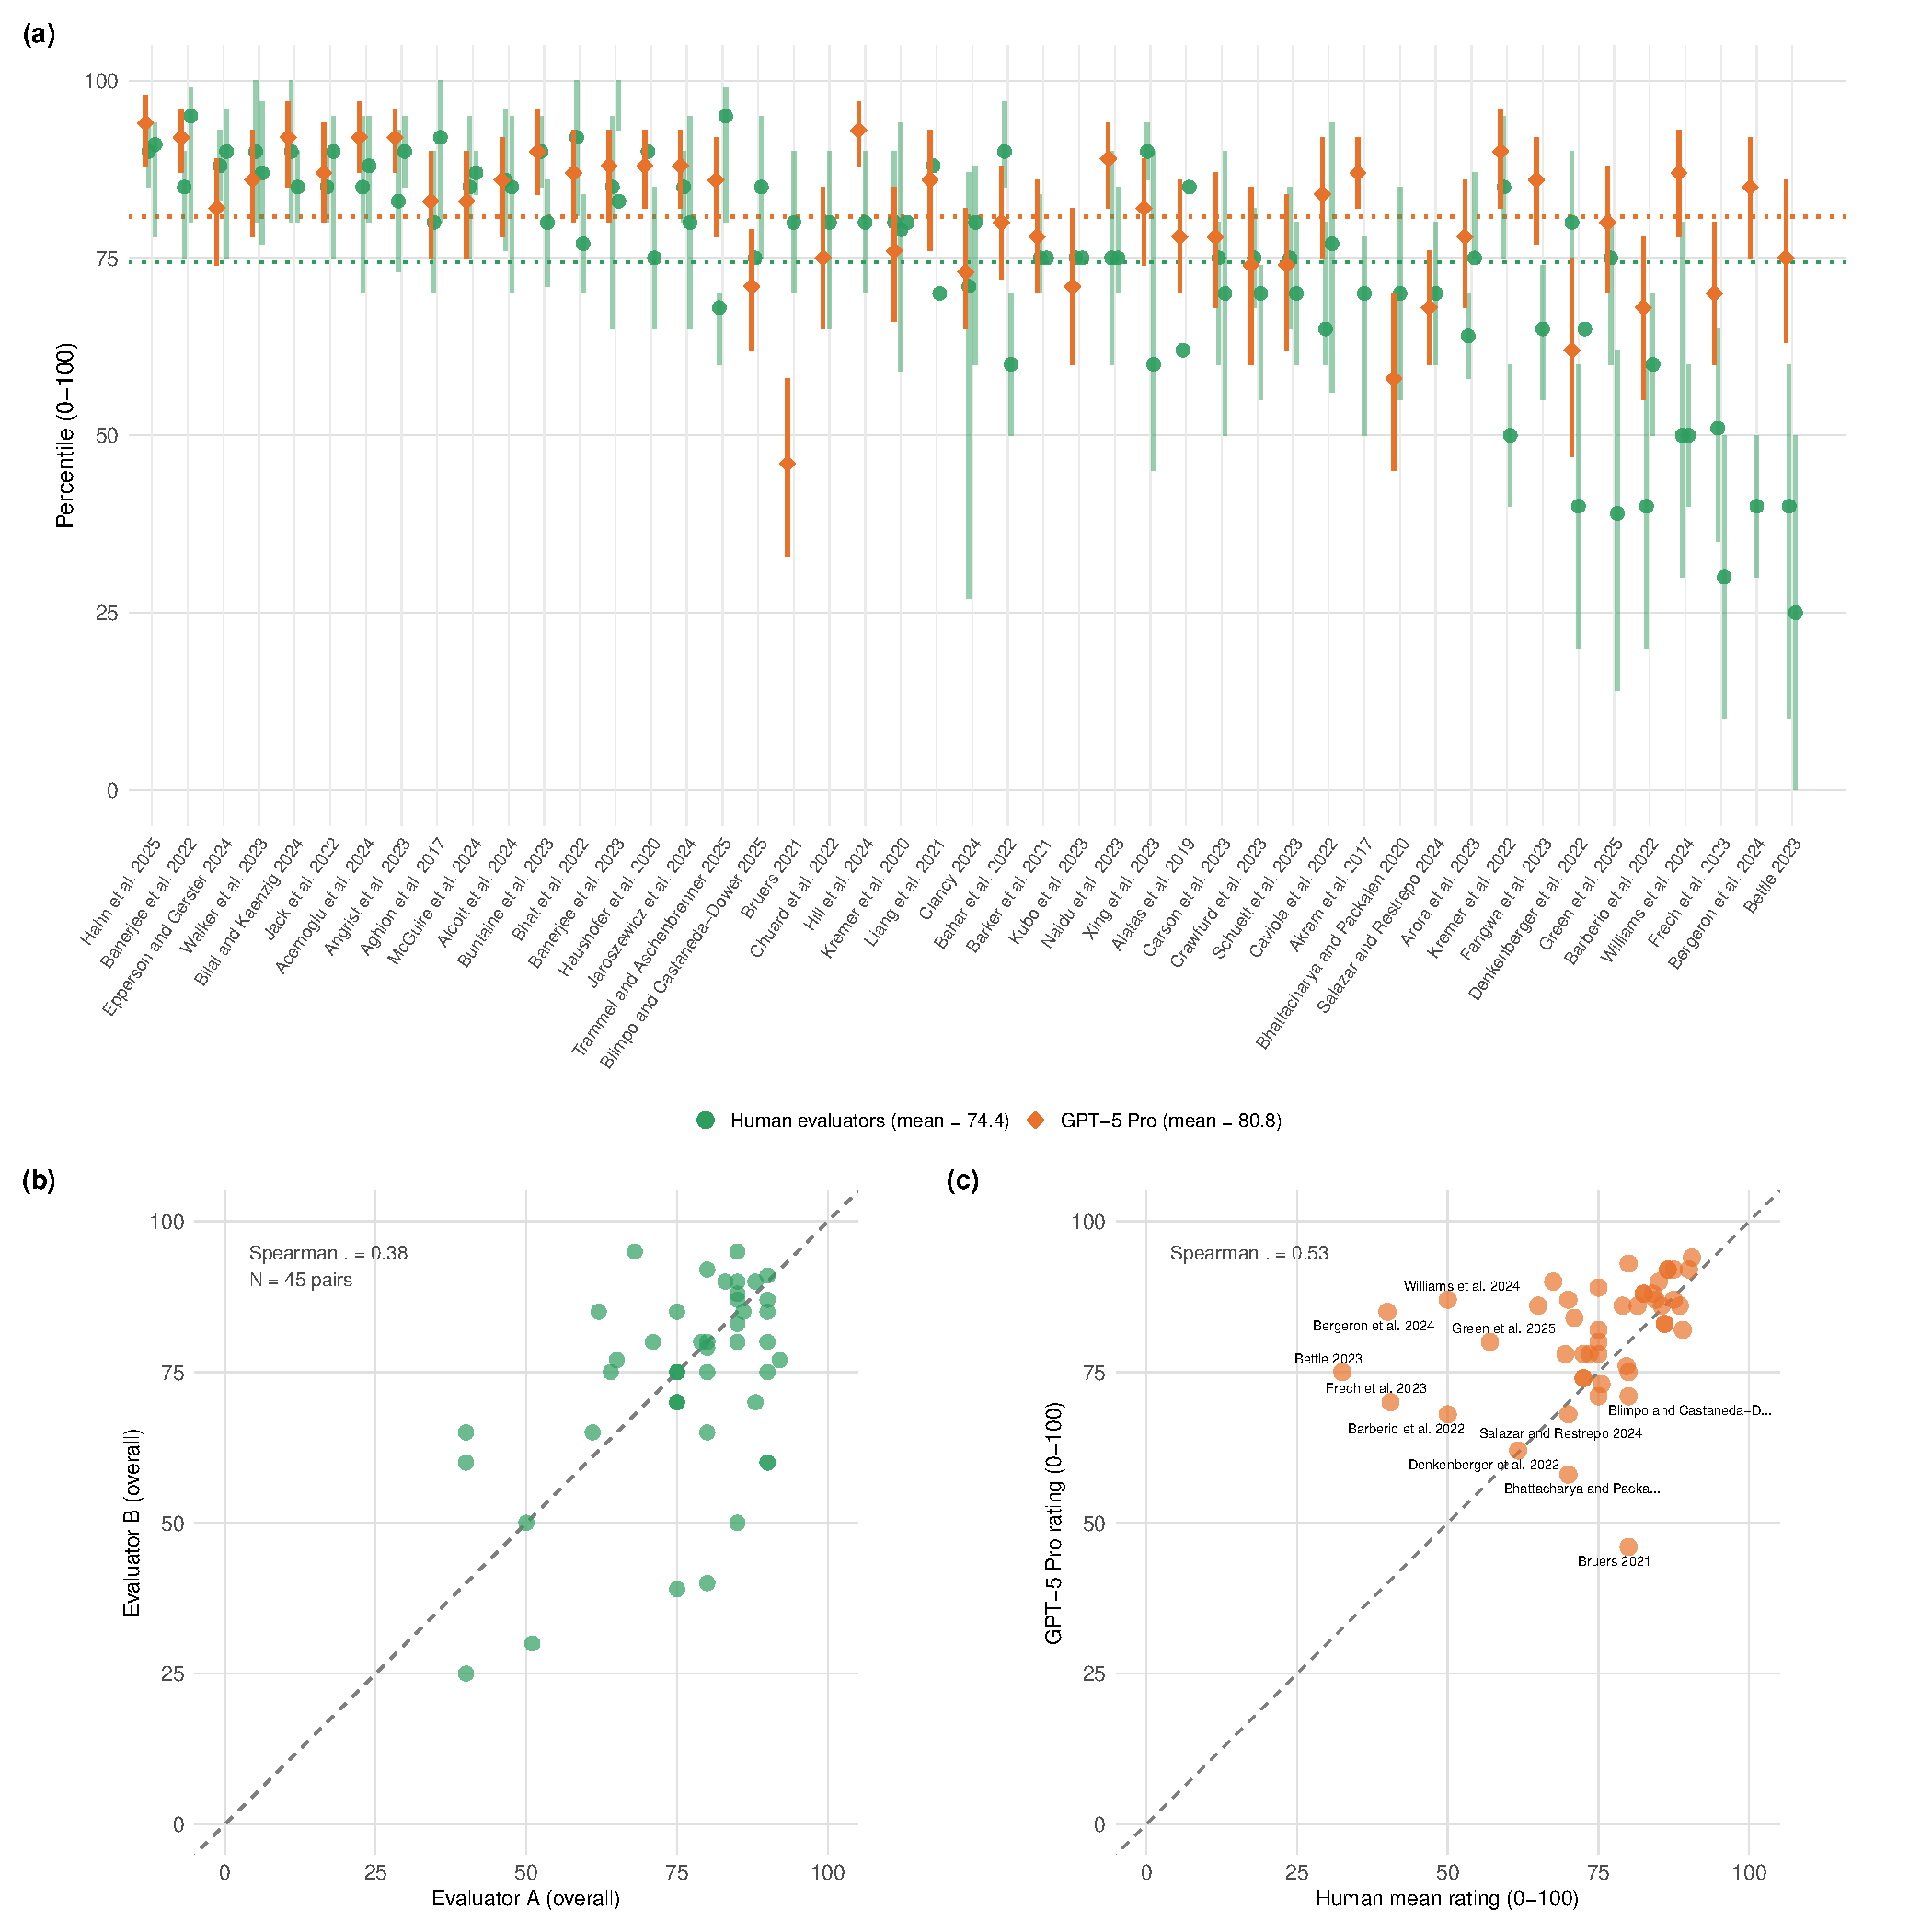
\includegraphics[keepaspectratio]{results_files/figure-pdf/fig-overview-combined-1.pdf}}

\end{figure}%

Panel (b) makes the human-human ceiling directly visible: the scatter of
evaluator pairs is no tighter than the GPT-5 Pro--human scatter in panel
(c), and individual pairs disagree by as much as 30--40 percentile
points on individual papers. GPT-5 Pro clusters around the identity line
in the 40--80 range but diverges more at the extremes, compressing
ratings toward the centre of the scale relative to humans---a pattern
consistent with alignment training that discourages extreme outputs.
Where humans rate a paper very highly or very harshly, the LLM typically
pulls toward the middle. Full agreement metrics for all six models
appear in \href{results_ratings.qmd}{Appendix A}.

\textbf{Rating differences by paper and criterion.}
Figure~\ref{fig-gap-heatmap-main} unpacks Human − GPT-5 Pro differences
across all seven criteria simultaneously. Each column is a paper, each
row a criterion, and tile colour encodes the signed difference (human
mean minus GPT-5 Pro midpoint). Green tiles indicate the human panel
rated the paper higher; orange tiles indicate GPT-5 Pro was more
generous. Papers are sorted by overall difference.

\begin{figure}

\caption{\label{fig-gap-heatmap-main}Human minus GPT-5 Pro rating
difference for every paper (columns) and criterion (rows). Green tiles
indicate the human mean was higher; orange tiles indicate GPT-5 Pro
rated the paper higher. Colour is clamped to ±30 percentile points.
Papers are sorted by overall difference.}

\pandocbounded{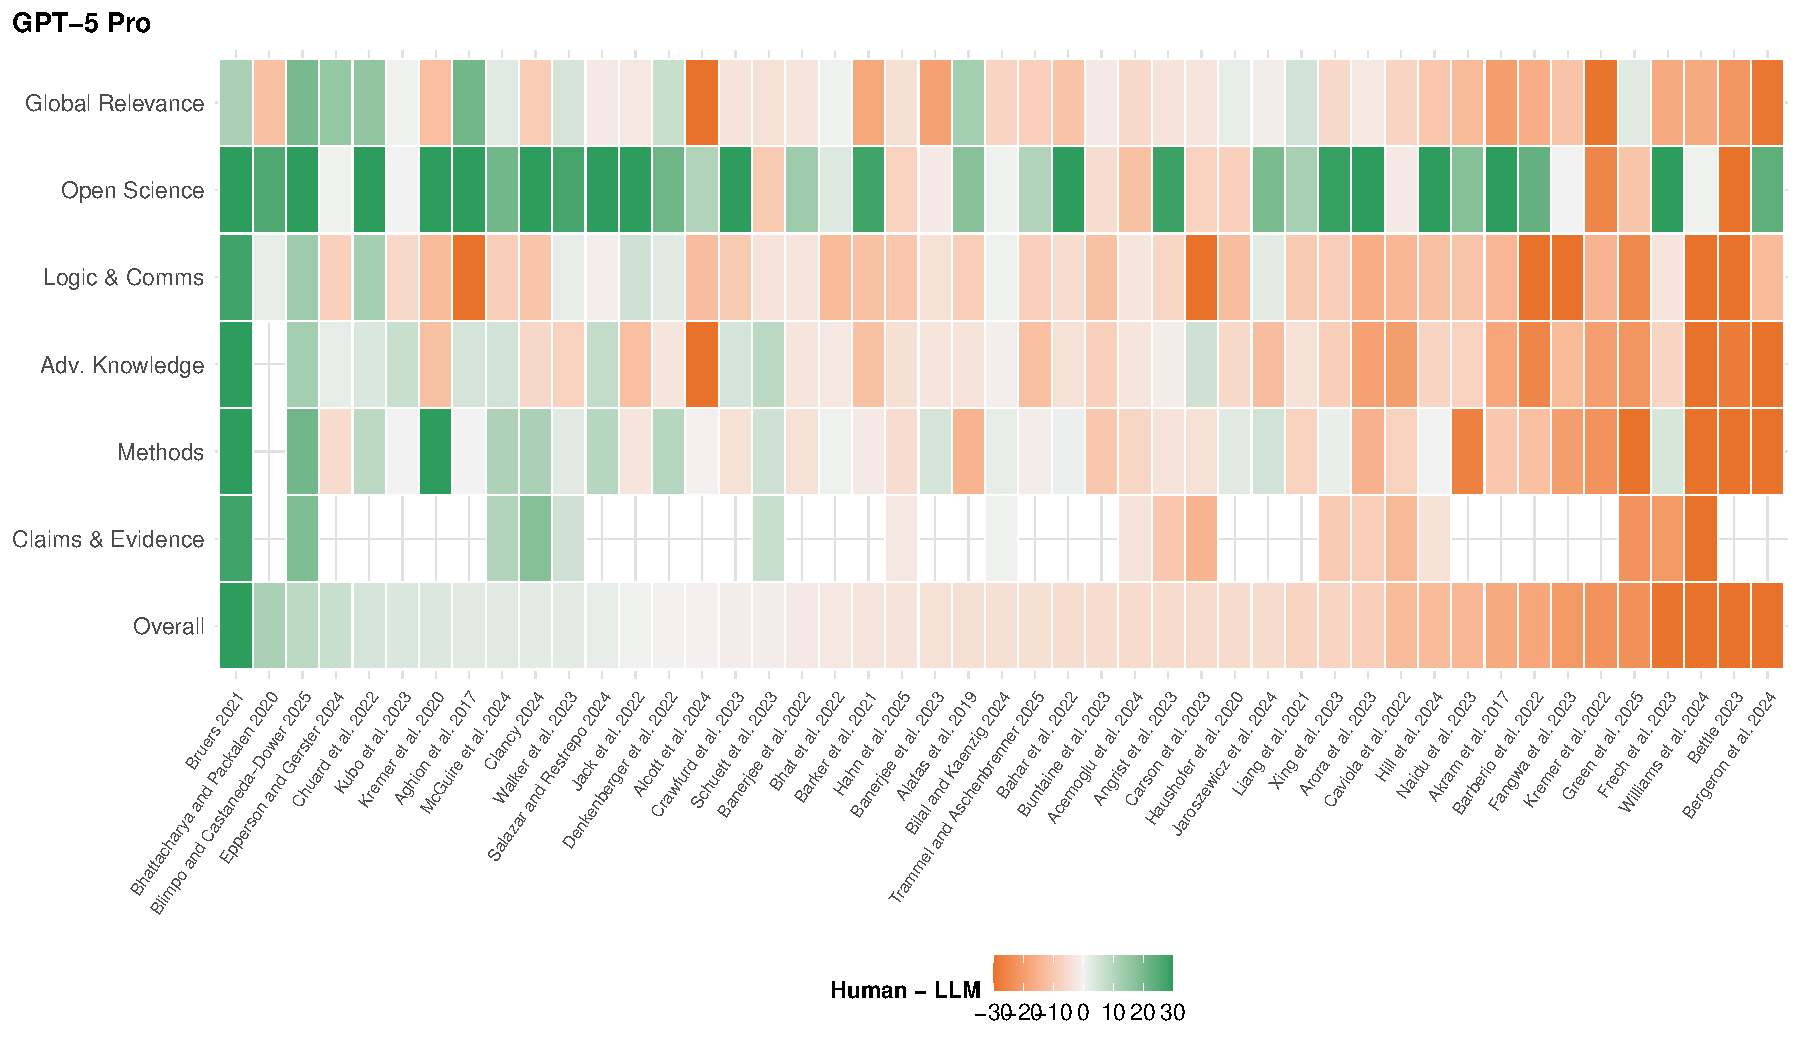
\includegraphics[keepaspectratio]{results_files/figure-pdf/fig-gap-heatmap-main-1.pdf}}

\end{figure}%

Rows with uniformly green or orange tiles indicate papers where humans
and GPT-5 Pro disagree systematically across all criteria, not just on
one dimension. Columns with consistent colour suggest criteria-level
biases---for instance, if ``Open Science'' is green across nearly all
papers, humans may systematically reward data-sharing practices more
than the model does. Multi-model comparisons in
\href{results_ratings.qmd}{Appendix A} reveal whether these disagreement
patterns are GPT-5 Pro--specific or shared across frontier LLMs.

\textbf{Qualitative critique comparison.} Beyond numeric ratings, we
compare the substantive critiques each model raises against the
consensus issues identified by human experts. The figure below plots
coverage---the fraction of human-identified concerns that the LLM also
raised in some form---against precision---the fraction of LLM-raised
issues that correspond to a substantive human concern. These metrics are
assessed by GPT-5.2 Pro acting as an independent judge (see
\href{methods.qmd}{Methods} for the judging protocol). One of the 14
originally curated pairs (Peterman et al.~2025) is excluded: the judge
flagged---and we verified against the paper---that the curated human
critique belonged to a different manuscript, so results are reported for
the remaining 13 pairs.

\begin{figure}

\caption{\label{fig-coverage-precision-main}Coverage (\% of
human-identified issues that the LLM also raised) vs Precision (\% of
LLM-raised issues that match a substantive human concern) for each
paper, as assessed by GPT-5.2 Pro acting as judge. Dashed lines mark the
cross-paper mean for each axis. Papers in the upper-right quadrant show
strong alignment between human and LLM critiques.}

\pandocbounded{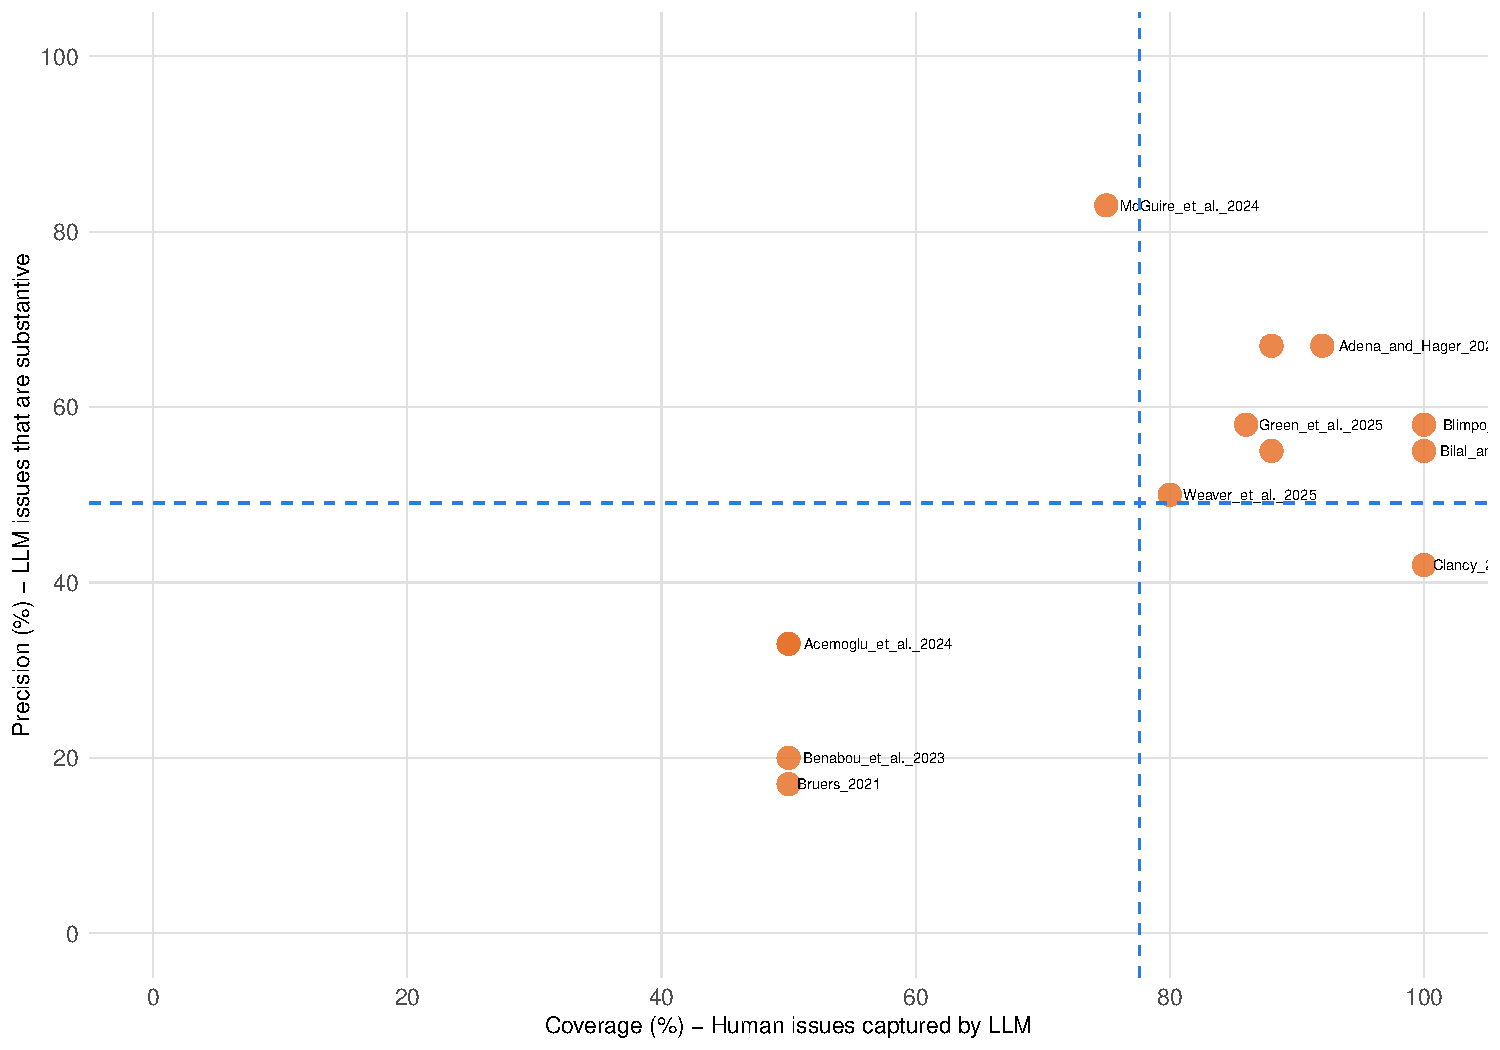
\includegraphics[keepaspectratio]{results_files/figure-pdf/fig-coverage-precision-main-1.pdf}}

\end{figure}%

Coverage and precision vary substantially across papers. Averaged over
the 13 focal papers, the model captures 78\% of human consensus issues
(range 50--100\%), while 49\% of model-raised issues match a substantive
human concern. Low precision partly reflects the reference set: the
human consensus list contains only the issues evaluation managers
prioritised, so model issues flagged by individual evaluators but not
curated into the consensus count against precision. Because these
metrics are themselves LLM-assessed, they should be interpreted with the
caveat that an LLM judge may systematically over- or under-credit
matches relative to a human annotator; the repository includes a
browser-based annotation tool for manual validation of these alignment
scores, which is ongoing.

Detailed paper-by-paper comparisons---including matched issue pairs with
severity labels, structural difference tables, and per-evaluator
breakdowns---appear in \href{results_critiques.qmd}{Appendix B:
Critiques \& Key Issues}. Extended quantitative analysis including all
six models, per-criterion correlations, bootstrap confidence intervals,
tier prediction accuracy, and cost-quality trade-offs is reported in
\href{results_ratings.qmd}{Appendix A: Results Ratings}. The full LLM
reasoning traces and assessment summaries are available in
\href{appendix_llm_traces.qmd}{Appendix C: LLM Traces}.

\textbf{Agreement summary.} Table~\ref{tbl-model-agreement-main} shows
GPT-5 Pro's agreement split into a \textbf{primary matched group} (same
39 papers as the H--H baseline, enabling like-for-like comparison) and a
\textbf{secondary full-sample group} (all 47 matched papers). In the
Spearman \emph{ρ} column, the H--H row shows individual-vs-individual
\emph{ρ} (the reference, already on the natural scale); GPT-5 Pro rows
show \emph{ρ} vs.~the human mean, which is upward-biased. The \textbf{ρ
adj.} column applies the Spearman-Brown correction to GPT-5 Pro rows
only, making them directly comparable to H--H \emph{ρ}. Six-model
comparison in \hyperref[tbl-agreement]{Appendix A, Table A2}.

\begin{longtable}[t]{lrrrrrrr}

\caption{\label{tbl-model-agreement-main}GPT-5 Pro overall-rating
agreement. \textbf{Primary (matched) group}: same 39 papers as the H-H
baseline (papers with at least 2 human raters). \textbf{Secondary
group}: all 47 matched papers. \textbf{Spearman rho column}: the H-H row
shows individual-vs-individual rank correlation (the reference, already
on the natural scale); GPT-5 Pro rows show correlation vs.~the human
mean, which is upward-biased relative to H-H. \textbf{rho adj.}:
Spearman-Brown corrected to the individual-rater equivalent (factor
0.83), making GPT-5 Pro rows directly comparable to H-H. \textbf{95\%
CI}: Fisher-z. Bias = LLM minus Human. Full six-model comparison in
\href{results_ratings.qmd}{Appendix A}.}

\tabularnewline

\toprule
Model & N & Spearman ρ & ρ adj. & 95\% CI & Pearson r & Mean bias & MAE\\
\midrule
\addlinespace[0.3em]
\multicolumn{8}{l}{\textcolor{black}{\textbf{Matched sample: same 39 papers as H-H baseline (primary)}}}\\
\hspace{1em}\cellcolor[HTML]{f0f8f0}{\textbf{Human-Human}} & \cellcolor[HTML]{f0f8f0}{\textbf{39}} & \cellcolor[HTML]{f0f8f0}{\textbf{0.331}} & \cellcolor[HTML]{f0f8f0}{\textbf{-}} & \cellcolor[HTML]{f0f8f0}{\textbf{{}[0.02, 0.59]}} & \cellcolor[HTML]{f0f8f0}{\textbf{0.520}} & \cellcolor[HTML]{f0f8f0}{\textbf{+3.7}} & \cellcolor[HTML]{f0f8f0}{\textbf{11.6}}\\
\hspace{1em}GPT-5 Pro & 39 & 0.627 & 0.520 & {}[0.39, 0.79] & 0.577 & +6.6 & 8.4\\
\addlinespace[0.3em]
\multicolumn{8}{l}{\textit{Full sample: all 47 GPT-5 Pro matched papers (secondary)}}\\
\hspace{1em}GPT-5 Pro & 47 & 0.526 & 0.436 & {}[0.28, 0.71] & 0.348 & +6.4 & 10.1\\
\bottomrule

\end{longtable}

The Fisher-z intervals in Table~\ref{tbl-model-agreement-main} quantify
uncertainty in each correlation separately; to make an uncertainty
statement about the \emph{comparison itself} we add a paired bootstrap
over papers (2,000 resamples of the 39 matched-group papers). Each draw
recomputes the GPT-5 Pro--human-mean rank correlation, applies that
draw's own Spearman-Brown correction, and takes the difference against
the human--human pairwise correlation on the same draw. The resulting
distribution of the adjusted difference (ρ adj. − ρ\textsubscript{HH})
spans {[}-0.11, 0.45{]}: the interval includes zero, so at this sample
size we cannot statistically separate the model from an additional human
rater---the two correlations are comparable, not demonstrably ordered.
This is the precise sense in which GPT-5 Pro ``performs within the human
inter-rater range.''

Table~\ref{tbl-criteria-agreement-main} breaks the same agreement
metrics down by evaluation criterion for GPT-5 Pro. The \textbf{H-H ρ}
column shows pairwise human-human Spearman ρ for each criterion as a
reference --- note that raw LLM ρ is upward-biased relative to H-H ρ by
the mean-vs-individual asymmetry (see
Table~\ref{tbl-model-agreement-main}). Criteria where H-H ρ is itself
low indicate genuine expert disagreement; low LLM agreement on those
criteria is therefore expected rather than a model failure.

\begin{longtable}[t]{l>{}rrrrr}

\caption{\label{tbl-criteria-agreement-main}GPT-5 Pro agreement with
human mean by criterion (N = 47 papers; N = 39 for H-H). \textbf{H-H
rho}: pairwise human evaluator rank correlation (reference; computed on
39 papers with at least 2 raters; raw LLM rho is upward-biased vs.~H-H
rho, see Table~\ref{tbl-model-agreement-main}). Positive bias = GPT-5
Pro rates higher on average. Note the variation across criteria: human
evaluators agree strongly on some dimensions and barely at all on others
(Open Science), setting expectations for LLM performance.}

\tabularnewline

\toprule
Criterion & H-H ρ & Spearman ρ & Pearson r & Mean bias & RMSE\\
\midrule
Overall & \textbf{0.331} & 0.526 & 0.348 & +6.4 & 15.1\\
Claims \& Evidence & \textbf{0.400} & 0.388 & 0.213 & +4.0 & 18.3\\
Methods & \textbf{0.375} & 0.562 & 0.356 & +4.5 & 18.1\\
Adv. Knowledge & \textbf{0.148} & 0.454 & 0.304 & +7.9 & 17.3\\
Logic \& Comms & \textbf{0.179} & 0.287 & 0.193 & +9.5 & 16.2\\
\addlinespace
Open Science & \textbf{-0.065} & 0.150 & 0.177 & -16.8 & 27.3\\
Global Relevance & \textbf{0.114} & 0.424 & 0.341 & +5.8 & 15.7\\
\bottomrule

\end{longtable}

\textbf{Journal-tier predictions and verifiable outcomes.} Beyond
percentile ratings, both evaluator types predict where each paper
\emph{will} publish on The Unjournal's 0--5 journal-tier scale. Unlike
percentile scores, these predictions eventually resolve against an
observable outcome: the venue where the paper actually publishes.

Human and GPT-5 Pro tier predictions agree at Spearman ρ = 0.75 (N = 42
papers with both predictions)---stronger agreement than on any
percentile criterion, suggesting that ``where will this publish'' is a
better-anchored question than ``what percentile is this paper.'' For 8
of these papers, The Unjournal's records already show a resolved
publication outcome that we can map to the tier scale
(Table~\ref{tbl-tier-outcomes}). On this small resolved set, mean
absolute error against the realized tier is 0.62 tiers for GPT-5 Pro and
0.71 for the human panel mean---both track outcomes to within roughly
two-thirds of a tier, and the sample is far too small to rank the two.

{

\begin{longtable}[]{@{}
  >{\raggedright\arraybackslash}p{(\linewidth - 8\tabcolsep) * \real{0.2039}}
  >{\raggedright\arraybackslash}p{(\linewidth - 8\tabcolsep) * \real{0.2913}}
  >{\raggedleft\arraybackslash}p{(\linewidth - 8\tabcolsep) * \real{0.1359}}
  >{\raggedleft\arraybackslash}p{(\linewidth - 8\tabcolsep) * \real{0.1650}}
  >{\raggedleft\arraybackslash}p{(\linewidth - 8\tabcolsep) * \real{0.2039}}@{}}

\caption{\label{tbl-tier-outcomes}Papers with resolved publication
outcomes: predicted vs realized journal tier (0--5 scale). Realized tier
maps The Unjournal's recorded publication status: `\textasciitilde top
journal' = 4.5, `decent journal' = 3.0, field journal = 2.5. Ambiguous
statuses, R\&R/forthcoming, and book chapters are treated as unresolved
and excluded. Human prediction is the evaluator mean.}

\tabularnewline

\toprule\noalign{}
\begin{minipage}[b]{\linewidth}\raggedright
Paper
\end{minipage} & \begin{minipage}[b]{\linewidth}\raggedright
Recorded outcome
\end{minipage} & \begin{minipage}[b]{\linewidth}\raggedleft
Realized tier
\end{minipage} & \begin{minipage}[b]{\linewidth}\raggedleft
Human prediction
\end{minipage} & \begin{minipage}[b]{\linewidth}\raggedleft
GPT-5 Pro prediction
\end{minipage} \\
\midrule\noalign{}
\endhead
\bottomrule\noalign{}
\endlastfoot
Alatas et al.~2019 & Published, \textasciitilde top journal & 4.5 & 3.50
& 3.9 \\
Barker et al.~2021 & Published, \textasciitilde top journal & 4.5 & 4.00
& 3.7 \\
Buntaine et al.~2023 & Published, \textasciitilde top journal & 4.5 &
4.70 & 4.5 \\
Hill et al.~2024 & Published, \textasciitilde top journal & 4.5 & 4.50 &
4.6 \\
Jack et al.~2022 & Published, \textasciitilde top journal & 4.5 & 4.00 &
4.5 \\
Fangwa et al.~2023 & published, decent journal & 3.0 & 3.60 & 4.0 \\
Kremer et al.~2020 & published, decent journal & 3.0 & 4.00 & 3.9 \\
Caviola et al.~2022 & Published: Psychology journal & 2.5 & 4.35 &
4.1 \\

\end{longtable}

}

Two caveats apply. First, most of these papers were published before the
model's training cutoff, so GPT-5 Pro may partly \emph{recall} venues
rather than predict them; human predictions were made before the
publication outcome was known, which makes this comparison structurally
generous to the model. Second, the remaining 34 papers with registered
predictions from both evaluator types are still unresolved (working
papers, R\&R, or forthcoming). These predictions are locked in this
repository and can be scored as outcomes accrue---a prospective
validation design that sidesteps the contamination concern entirely,
since future publication decisions cannot appear in any current model's
training data.

All appendices, interactive figures, and full code are available at the
companion website: \url{https://llm-uj-research-eval.netlify.app}.
Source code and data are hosted at
\url{https://github.com/valentinklotzbuecher/llm-uj-research-eval}.

\bookmarksetup{startatroot}

\section{Discussion}\label{discussion}

GPT-5 Pro achieves moderate-to-strong agreement with human expert
evaluators: a paired bootstrap cannot distinguish its rank agreement
with the human panel from the agreement observed between human
evaluators themselves. Central compression---the tendency to pull
extreme ratings toward the middle of the scale---is the most consistent
pattern, likely reflecting alignment training that discourages confident
extreme outputs. Journal-tier predictions are the dimension where human
and model judgments align most closely, and on the small set of papers
whose publication outcomes have already resolved, both predict realized
venues with broadly similar accuracy. Qualitative coverage varies widely
across papers: on some, the model captures nearly all consensus human
concerns; on others, it misses key critiques or raises issues absent
from the expert consensus. Appendix results for five additional models
confirm these patterns across capability tiers, with reasoning-capable
models outperforming lightweight ones.

\textbf{Limitations.} Several caveats temper these conclusions. Our
sample comprises 60 social-science papers evaluated by the model, of
which 47 have published human evaluation packages for direct comparison;
all were specifically selected by The Unjournal for evaluation, not a
random draw from the research literature; performance may differ in
other fields or on less polished manuscripts. Human evaluations are
themselves a noisy reference signal rather than ground truth, with
substantial inter-rater variation that caps achievable agreement. We
cannot fully rule out knowledge contamination: while we instruct the
model to ignore prior knowledge about authors, institutions, or
publication history in the system prompt, the models' training data may
include fragments of these papers or related discussions. Robustness
checks with models whose training cutoffs predate the papers, or
out-of-time validation on papers entering The Unjournal's pipeline after
model training, would help address this concern. Alignment training
likely contributes to score inflation and narrower credible intervals
than humans provide. All LLM evaluations are single-run; aggregating
across multiple runs or temperature settings could change the picture.
Finally, the qualitative coverage and precision metrics are themselves
LLM-assessed (GPT-5.2 Pro as judge), introducing a further layer of
model dependence.

\textbf{Implications.} Even a reasoning-capable model costing several
dollars per paper is orders of magnitude cheaper than human expert
review. The qualitative gaps we observe---missed critiques, generic
issues, and central compression of ratings---argue against full
automation of peer review. AI evaluation appears most promising as a
supplement: providing fast structured feedback, flagging potential
concerns for human reviewers, and enabling systematic comparison across
large paper sets that would be infeasible with human effort alone.

\textbf{Governance and attack surface.} As AI review tools move from
research prototypes to deployed products, the attack surface expands.
Prompt-injection techniques---embedding hidden instructions in a
manuscript's metadata, footnotes, or even white-on-white text---could
steer model outputs toward inflated ratings or suppressed critiques.
Because our pipeline (and similar commercial services) routes
unpublished manuscripts through third-party APIs, confidentiality cannot
be guaranteed without end-to-end encryption or on-premise deployment.
Over-reliance on AI scores introduces a further governance risk: if
editorial decisions weight model ratings, authors may optimise papers
for the model rather than for scientific rigour, creating a Goodhart
dynamic. Finally, current evaluations reflect a single model checkpoint;
model updates, alignment changes, or fine-tuning can shift ratings in
ways that are invisible to users. We recommend that any operational
deployment include adversarial red-teaming of prompts, formal
confidentiality agreements with API providers, transparent disclosure of
AI involvement in review, and periodic re-calibration against fresh
human evaluations.

\textbf{Future directions.} All LLM evaluations reported here are
single-run; multi-run robustness and prompt-sensitivity analysis would
directly address the key open methodological question. Out-of-time
validation on papers entering The Unjournal's pipeline after model
training cutoffs would eliminate residual contamination concerns. The
qualitative coverage and precision metrics are themselves LLM-assessed
(GPT-5.2 Pro as judge); human validation of these scores is needed to
close the model-dependence loop. Finally, the tier-prediction comparison
in Results is a first step toward externally verifiable accuracy
measurement: roughly thirty papers with registered predictions from both
evaluator types have not yet resolved, and scoring those predictions as
publication outcomes accrue provides a contamination-free horse race
that strengthens with time.

\bookmarksetup{startatroot}

\section{Methods}\label{methods}

\small

This chapter describes the data sources, evaluation pipeline, prompt
design, and statistical methods used throughout. All Python code
underlying the pipeline is preserved in the collapsible blocks below and
can be executed to reproduce the evaluation runs.

\textbf{Sample and human reference data.} We draw on published
evaluations from
\href{https://unjournal.github.io/unjournaldata/index.html}{The
Unjournal}, an open-access platform that commissions expert reviews of
policy-relevant research without requiring journal submission. Each
paper is typically assessed by two independent evaluators (occasionally
one or three), who provide a written critique resembling a referee
report together with quantitative ratings on seven criteria scored as
percentiles (0--100) relative to ``all serious research in the same area
encountered in the last three years.''\footnote{The seven criteria are:
  \emph{overall assessment}, \emph{claims and evidence}, \emph{methods},
  \emph{advancing knowledge and practice}, \emph{logic and
  communication}, \emph{open and collaborative science}, and
  \emph{relevance to global priorities}. Full definitions are given in
  The Unjournal's
  \href{https://globalimpact.gitbook.io/the-unjournal-project-and-communication-space/policies-projects-evaluation-workflow/evaluation/guidelines-for-evaluators}{guidelines
  for evaluators}.} Evaluators additionally predict the journal tier in
which the work ``should'' and ``will'' publish, using a 0--5 continuous
scale anchored to familiar venue categories (0 = unpublishable, 5 =
top-5 journal). For each metric, evaluators report a midpoint (median of
their belief distribution) and a 90\% credible interval that expresses
their epistemic uncertainty.

The sample comprises working papers spanning 2017--2025 in development
economics, health policy, environmental economics, and related fields
that The Unjournal identified as high-impact. All papers have completed
The Unjournal's full evaluation process, meaning the authors received
evaluations that have been publicly posted. For our analysis we
extracted the individual evaluator scores, aggregated them by taking the
arithmetic mean per paper per criterion, and retained the range of
individual scores to characterise inter-rater spread.

\textbf{LLM evaluation pipeline.} We evaluate six frontier models
spanning three providers: GPT-5 Pro and GPT-5.2 Pro (OpenAI,
reasoning-capable), GPT-4o-mini (OpenAI, lightweight), Claude Sonnet 4
and Claude Opus 4.6 (Anthropic), and Gemini 2.0 Flash (Google). Each
model receives the identical PDF file, system prompt, and output schema.
We pass the PDF directly to the model's native multimodal input rather
than extracting text, preserving tables, figures, equations, and layout
cues that ad-hoc scraping could mangle. A single API call per paper
avoids hand-offs and summary loss from multi-stage pipelines.

The output is constrained by a strict JSON Schema enforcing the same
nine fields that human evaluators complete: seven percentile metrics
(each with \texttt{midpoint}, \texttt{lower\_bound},
\texttt{upper\_bound}) and two journal-tier predictions (each with
\texttt{score}, \texttt{ci\_lower}, \texttt{ci\_upper}). Additionally,
the model produces an \texttt{assessment\_summary} of approximately
1,000 words that must precede scoring---a ``think first, score second''
protocol designed to ground numeric ratings in specific textual
evidence. The extended schema used for our GPT-5.2 Pro focal run adds a
\texttt{key\_issues} array of concise, ranked issue statements for
downstream critique comparison.

\textbf{Agreement and reliability statistics.} We quantify human--LLM
agreement using several complementary measures. \emph{Pearson's r}
captures linear association between paired ratings and is sensitive to
proportional biases but not to constant offsets. \emph{Spearman's ρ}
measures rank-order agreement and is robust to outliers and non-linear
monotone relationships. \emph{Mean bias} (LLM minus human) indicates the
direction and magnitude of any systematic offset. \emph{Root mean
squared error} (RMSE) and \emph{mean absolute error} (MAE) measure
typical prediction error in the original scale units; RMSE penalises
large deviations more heavily. To contextualise human--LLM agreement we
report \emph{Krippendorff's alpha} (\(\alpha\)), a chance-corrected
reliability coefficient that generalises across varying numbers of
raters, accommodates missing data, and applies to any measurement level
(nominal, ordinal, interval, or ratio). An \(\alpha\) of 1 indicates
perfect agreement, 0 indicates agreement no better than chance, and
values below 0 indicate systematic disagreement. We compute
\(\alpha_{\text{HH}}\) (among human evaluators only) as a ceiling: if
human evaluators agree with each other at only \(\alpha = 0.5\) on a
given criterion, expecting an LLM to exceed that level would be
unrealistic. We then report \(\alpha_{\text{HL}}\) (between the human
mean and each LLM) to assess how close machine ratings come to this
ceiling. For the qualitative key-issue comparison, \emph{coverage}
denotes the fraction of human-identified issues that received a match
score \(\geq 30\%\) from the LLM judge, and \emph{precision} denotes the
fraction of LLM-generated issues that matched at least one human issue.

\textbf{JSON Schema.} The output schema enforces that every paper is
scored on identical fields with identical types and bounds. Credible
intervals are required (paralleling the human protocol) so that the
model can express genuine uncertainty rather than suggest false
precision.

\textbf{System prompt design.} The system prompt is assembled from
modular components and concatenated before each API call. It opens with
a role definition instructing the model to act as an expert research
evaluator, followed by a debiasing block that explicitly prohibits use
of author identity, institutional prestige, publication venue, or any
extrinsic information---the model must base all judgments on the PDF
content alone. A diagnostic-summary instruction requires the model to
produce a roughly 1,000-word assessment identifying methodological,
evidential, and interpretive issues \emph{before} any scoring,
implementing a ``think first, score second'' protocol intended to anchor
numeric ratings in specific textual evidence.

Percentile ratings are anchored to the reference group ``all serious
research in the same area encountered in the last three years,''
following The Unjournal's
\href{https://globalimpact.gitbook.io/the-unjournal-project-and-communication-space/policies-projects-evaluation-workflow/evaluation/guidelines-for-evaluators}{guidelines
for evaluators}. The prompt defines each of the seven criteria with
emphasis on global priorities and practical relevance over pure academic
novelty, mirroring the weight structure that human Unjournal evaluators
are asked to apply.

Subsequent prompt components instruct the model on constructing 90\%
credible intervals---the smallest interval the evaluator believes is
90\% likely to contain the true value---encouraging calibrated
uncertainty rather than artificially narrow bounds. The prompt requests
journal-tier predictions on a 0--5 continuous scale anchored to familiar
venue categories (0 = unpublishable through 5 = top-5 journal),
providing an externally verifiable reference point for papers that
eventually publish. A validation block then requires the model to verify
internal consistency: numeric scores must align with the written
assessment, credible intervals must be non-degenerate, and high or low
ratings must be explicitly justified in the assessment summary.

The components above are concatenated into a single system prompt string
before each API call:

\textbf{Submission and collection.} The \texttt{evaluate\_paper}
function uploads a PDF to the API and submits a background job for
evaluation. File IDs are cached by path, size, and modification time so
that re-running on the same PDF reuses the previously uploaded file.

Each model receives the full PDF in a single reasoning call, avoiding
hand-offs and summary loss from multi-stage ingestion. We submit one
background job per paper to the OpenAI Responses API with ``high''
reasoning effort and server-side JSON-Schema enforcement, recording the
response ID, model, file ID, status, and timestamps in a jobs index. No
external sources or cross-paper material are retrieved; the evaluation
is anchored entirely in the manuscript itself.

A polling loop then checks each job's status and, for completed jobs,
retrieves the raw JSON response object and writes it to disk alongside
reasoning-trace metadata (token counts, reasoning summary).

\textbf{Multi-model evaluation.} To assess whether systematic biases or
calibration differences emerge across architectures, we collect
evaluations from six models spanning three providers. For OpenAI models
that lack background-job or extended-reasoning support (e.g.,
GPT-4o-mini), we use a synchronous call variant:

\textbf{Anthropic.} Anthropic's API accepts PDFs as base64-encoded
document content rather than uploaded file IDs, and all calls are
synchronous. We use Claude's native PDF support to preserve the same
multimodal evaluation approach:

\textbf{Google.} Google's Gemini API accepts PDFs via a file-upload
endpoint with MIME-type tagging:

A unified runner dispatches evaluations across all configured providers
and writes per-model output directories:

\textbf{Focal run with key-issue extraction.} For a subset of 14 papers
with rich human critiques, we ran an extended evaluation using GPT-5.2
Pro. The schema for this focal run adds a \texttt{key\_issues} array---a
ranked list of concise issue statements identifying the most important
methodological, interpretive, or evidential concerns---alongside the
standard metrics. This structured output enables direct comparison
between machine-generated and human-identified issues. One curated pair
(Peterman et al.~2025) was later excluded from the comparison after the
LLM judge flagged, and we verified, that its human critique had been
misattributed to a different manuscript during curation; the
coverage/precision analysis therefore covers 13 papers.

\textbf{Key-issue comparison with human critiques.} To validate how well
the LLM identifies substantive concerns, we compare its
\texttt{key\_issues} output against human expert critiques drawn from
The Unjournal's Coda database. These human critiques---produced by paid
domain experts and synthesized by evaluation managers---provide a
high-quality but noisy reference standard for issue identification;
accordingly, we treat them as a comparative signal rather than ground
truth.

The comparison proceeds in two stages. First, we parse and align the
data sources: LLM key issues are extracted from the focal-run JSON
responses, while human critiques are drawn from a manually curated
markdown document pairing each paper's machine and expert assessments.
Second, we use an LLM judge (GPT-5.2 Pro with schema-enforced structured
output) to systematically assess the degree of alignment between each
human-identified issue and the set of machine-generated issues,
producing issue-by-issue match scores, coverage estimates (fraction of
human issues captured), and precision estimates (fraction of LLM issues
that are genuinely substantive).

The comparison pipeline takes a manually curated markdown file pairing
each paper's LLM issues with human critiques and produces two structured
outputs: a parsed JSON dataset (\texttt{key\_issues\_comparison.json})
and an LLM-assessed alignment report
(\texttt{key\_issues\_comparison\_results.json}) containing per-paper
coverage, precision, matched-pair explanations, and an overall quality
rating. Together, these outputs feed the qualitative analysis presented
in \href{results_critiques.qmd}{Appendix B: Critiques \& Key Issues}.

\normalsize

\bookmarksetup{startatroot}

\section*{References}\label{references}
\addcontentsline{toc}{section}{References}

\markboth{References}{References}

\protect\phantomsection\label{refs}
\begin{CSLReferences}{1}{0}
\bibitem[\citeproctext]{ref-aczel2021billion}
Aczel, Balazs, Barnabas Szaszi, and Alex O Holcombe, {``A billion-dollar
donation: Estimating the cost of researchers' time spent on peer
review,''} \emph{Research integrity and peer review}, 6 (2021), 1--8
(Springer).

\bibitem[\citeproctext]{ref-AsherMalzahnPersanoPaschalMyersHall2026P_Hack}
Asher, Samuel G. Z., Janet Malzahn, Jessica M. Persano, Elliot J.
Paschal, Andrew C. W. Myers, and Andrew B. Hall, {``Do claude code and
codex p-hack? {Sycophancy} and statistical analysis in large language
models,''} 2026.

\bibitem[\citeproctext]{ref-AsirvathamMokskiShleifer2026GPTMeasurement}
Asirvatham, Hemanth, Elliott Mokski, and Andrei Shleifer,
{``\href{https://www.nber.org/papers/w34834}{{GPT} as a measurement
tool},''} \{NBER\} Working Paper, 2026 (National Bureau of Economic
Research).

\bibitem[\citeproctext]{ref-choi2026invisible}
Choi, Byungjin, Tae Joon Jun, Joung Won Sung, Il Woo Park, Jeong-Moo
Lee, Soo Ick Cho, Hyung Jun Park, Ro Woon Lee, and Jungyo Suh,
{``\href{https://doi.org/10.1001/jamanetworkopen.2025.52099}{Invisible
text injection and peer review by AI models},''} \emph{JAMA Network
Open}, 9 (2026), e2552099.

\bibitem[\citeproctext]{ref-elsevierAIPolicy2025}
Elsevier, {``Generative AI policies for journals,''}
\textless{}\url{https://www.elsevier.com/about/policies-and-standards/generative-ai-policies-for-journals}\textgreater{}
(Feb. 19, 2026).

\bibitem[\citeproctext]{ref-openAIReview2026}
Hsu, Chao-Chun, and Chenhao Tan,
{``\href{https://openaireview.github.io/blog.html}{OpenAIReview:
Open-source AI-assisted academic paper reviewing},''} 2026.

\bibitem[\citeproctext]{ref-isitcredible}
IsItCredible.com, {``Is it credible?''}
\textless{}\url{https://www.isitcredible.com/}\textgreater{} (Feb. 19,
2026).

\bibitem[\citeproctext]{ref-leung2026policies}
Leung, Tiffany I.,
{``\href{https://doi.org/10.1001/jamanetworkopen.2025.52042}{LLMs in
peer review---how publishing policies must advance},''} \emph{JAMA
Network Open}, 9 (2026), e2552042.

\bibitem[\citeproctext]{ref-qedScience2026}
QED Science, {``\href{https://www.qedscience.com/}{QED science: Critical
thinking AI for research},''} 2026.

\bibitem[\citeproctext]{ref-rajakumar2026peerreview}
Rajakumar, Hamrish Kumar, Kailash Abhishek Sankaran, Manasi Pillai
Ashok, and Srinivas Rachoori,
{``\href{https://doi.org/10.1093/postmj/qgag005}{Peer review in the age
of artificial intelligence: A comparative study of human and
AI-generated review reports},''} \emph{Postgraduate Medical Journal},
(2026), qgag005.

\bibitem[\citeproctext]{ref-refineFAQ}
Refine, {``FAQ - refine,''}
\textless{}\url{https://www.refine.ink/faq}\textgreater{} (Feb. 19,
2026).

\bibitem[\citeproctext]{ref-spitzer2026submission}
Spitzer, Markus Wolfgang Hermann,
{``\href{https://doi.org/10.1016/j.tine.2026.100276}{The emerging
submission crisis in behavioral science},''} \emph{Trends in
Neuroscience and Education}, 42 (2026), 100276.

\bibitem[\citeproctext]{ref-thomas2026jagged}
Thomas, Llewellyn D. W., Angelo Kenneth G. Romasanta, and Laia Pujol
Priego, {``\href{https://doi.org/10.1016/j.jbusres.2025.115804}{Jagged
competencies: Measuring the reliability of generative AI in academic
research},''} \emph{Journal of Business Research}, 203 (2026), 115804.

\bibitem[\citeproctext]{ref-wang2025psychometric}
Wang, Yuehan, Jinyan Huang, Lun Du, Yuxin Guo, Ying Liu, and Rong Wang,
{``\href{https://doi.org/10.1016/j.caeai.2025.100481}{Evaluating large
language models as raters in large-scale writing assessments: A
psychometric framework for reliability and validity},''} \emph{Computers
and Education: Artificial Intelligence}, 9 (2025), 100481.

\bibitem[\citeproctext]{ref-Zhang2025}
Zhang, Tianmai M, and Neil F Abernethy,
{``\href{https://arxiv.org/abs/2505.23824v2}{Reviewing scientific papers
for critical problems with reasoning LLMs: Baseline approaches and
automatic evaluation},''} \emph{arXiv preprint arXiv:2505.23824},
(2025).

\end{CSLReferences}

\cleardoublepage
\phantomsection
\addcontentsline{toc}{part}{Appendices}
\appendix

\section{Results: Ratings}\label{results-ratings}

Extended ratings analysis (per-criterion correlations, agreement
metrics, human baseline, cost--quality trade-offs) is available in the
online supplement at
\url{https://llm-uj-research-eval.netlify.app/results_ratings.html}.

\section{Results: Critiques \& Key
Issues}\label{results-critiques-key-issues}

Detailed paper-by-paper critique comparisons (matched issue pairs,
severity labels, structural differences) are available in the online
supplement at
\url{https://llm-uj-research-eval.netlify.app/results_critiques.html}.

\section{Supplementary Material}\label{supplementary-material}

Full LLM reasoning traces, assessment summaries, related work, and
extended analyses are available in the online supplement at
\url{https://llm-uj-research-eval.netlify.app/appendix_llm_traces.html}.

\section{Did Authors Respond to Unjournal
Evaluations?}\label{did-authors-respond-to-unjournal-evaluations}

The interactive tables in this appendix are available in the online
version at
\url{https://valentinklotzbuecher.github.io/llm-uj-research-eval/paper_response_analysis.html}.

\begin{tcolorbox}[enhanced jigsaw, arc=.35mm, bottomrule=.15mm, bottomtitle=1mm, breakable, colback=white, colbacktitle=quarto-callout-note-color!10!white, colframe=quarto-callout-note-color-frame, coltitle=black, left=2mm, leftrule=.75mm, opacityback=0, opacitybacktitle=0.6, rightrule=.15mm, title=\textcolor{quarto-callout-note-color}{\faInfo}\hspace{0.5em}{Note}, titlerule=0mm, toprule=.15mm, toptitle=1mm]

57 Unjournal evaluations tracked as of April 2026, drawing on two
evidence streams: (a) manual staff assessment of author responses and
paper revisions; (b) Claude Opus 4.6 change-attribution for 8 papers
where pre/post PDFs were available. See
\hyperref[combined-evidence]{Combined Evidence} below.

\end{tcolorbox}

\subsection{Overview}\label{overview}

The Unjournal commissions open, structured evaluations of working papers
in economics and social science. A natural question is whether this
process changes research: do authors engage with feedback and revise
their work?

This page draws on manual classification of 57 tracked evaluations and,
for a subset, automated PDF diffing and LLM attribution. Background:
\href{https://globalimpact.gitbook.io/the-unjournal-project-and-communication-space/benefits-and-features/more-reliable-and-useful-evaluation/author-engagement-evidence}{The
Unjournal's knowledge base}.

\begin{Shaded}
\begin{Highlighting}[]
\FunctionTok{library}\NormalTok{(dplyr)}
\FunctionTok{library}\NormalTok{(ggplot2)}
\FunctionTok{library}\NormalTok{(readr)}
\FunctionTok{library}\NormalTok{(DT)}
\FunctionTok{library}\NormalTok{(tidyr)}
\FunctionTok{library}\NormalTok{(stringr)}
\FunctionTok{library}\NormalTok{(glue)}
\FunctionTok{library}\NormalTok{(jsonlite)}

\NormalTok{df }\OtherTok{\textless{}{-}} \FunctionTok{read\_csv}\NormalTok{(}\StringTok{"data/author\_adjustment\_manual.csv"}\NormalTok{, }\AttributeTok{show\_col\_types =} \ConstantTok{FALSE}\NormalTok{)}

\NormalTok{df }\OtherTok{\textless{}{-}}\NormalTok{ df }\SpecialCharTok{|\textgreater{}}
  \FunctionTok{rename}\NormalTok{(}
    \AttributeTok{paper\_title    =}\NormalTok{ label\_paper\_title,}
    \AttributeTok{pubpub\_link    =}\NormalTok{ dup\_pubpub\_final\_links,}
    \AttributeTok{adj\_status     =} \StringTok{\textasciigrave{}}\AttributeTok{Adjusted\_paper?}\StringTok{\textasciigrave{}}\NormalTok{,}
    \AttributeTok{updated\_manual =} \StringTok{\textasciigrave{}}\AttributeTok{Updated since UJ report {-}{-} manual confirmation}\StringTok{\textasciigrave{}}\NormalTok{,}
    \AttributeTok{deposit\_after  =} \StringTok{\textasciigrave{}}\AttributeTok{deposit date \textgreater{} unjournal pub date}\StringTok{\textasciigrave{}}\NormalTok{,}
    \AttributeTok{research\_area  =}\NormalTok{ main\_cause\_cat\_abbrev,}
    \AttributeTok{nb\_link        =}\NormalTok{ notebookLM\_link,}
    \AttributeTok{pub\_status     =}\NormalTok{ publication\_status,}
    \AttributeTok{wp\_date        =}\NormalTok{ working\_paper\_release\_date,}
    \AttributeTok{uj\_pub\_date    =}\NormalTok{ publication\_date\_unjournal}
\NormalTok{  )}

\NormalTok{adj\_labels }\OtherTok{\textless{}{-}} \FunctionTok{c}\NormalTok{(}
  \StringTok{"Evidence of updating"}\NormalTok{, }\StringTok{"Stated intention to update"}\NormalTok{,}
  \StringTok{"Mixed / minor updating"}\NormalTok{, }\StringTok{"Unlikely to update"}\NormalTok{, }\StringTok{"Not yet assessed"}
\NormalTok{)}

\NormalTok{df }\OtherTok{\textless{}{-}}\NormalTok{ df }\SpecialCharTok{|\textgreater{}}
  \FunctionTok{mutate}\NormalTok{(}
    \AttributeTok{adj\_status\_clean =} \FunctionTok{case\_when}\NormalTok{(}
\NormalTok{      adj\_status }\SpecialCharTok{==} \StringTok{"evidence of updating"}          \SpecialCharTok{\textasciitilde{}} \StringTok{"Evidence of updating"}\NormalTok{,}
\NormalTok{      adj\_status }\SpecialCharTok{==} \StringTok{"Stated intention to update"}    \SpecialCharTok{\textasciitilde{}} \StringTok{"Stated intention to update"}\NormalTok{,}
\NormalTok{      adj\_status }\SpecialCharTok{==} \StringTok{"mixed evidence/minor updating"} \SpecialCharTok{\textasciitilde{}} \StringTok{"Mixed / minor updating"}\NormalTok{,}
\NormalTok{      adj\_status }\SpecialCharTok{==} \StringTok{"Unlikely to update"}            \SpecialCharTok{\textasciitilde{}} \StringTok{"Unlikely to update"}\NormalTok{,}
      \ConstantTok{TRUE}                                          \SpecialCharTok{\textasciitilde{}} \StringTok{"Not yet assessed"}
\NormalTok{    ),}
    \AttributeTok{adj\_status\_clean =} \FunctionTok{factor}\NormalTok{(adj\_status\_clean, }\AttributeTok{levels =}\NormalTok{ adj\_labels),}
    \AttributeTok{author\_response\_clean =} \FunctionTok{case\_when}\NormalTok{(}
\NormalTok{      author\_response }\SpecialCharTok{==} \StringTok{"Formal response"} \SpecialCharTok{\textasciitilde{}} \StringTok{"Formal response"}\NormalTok{,}
\NormalTok{      author\_response }\SpecialCharTok{==} \StringTok{"Informal"}        \SpecialCharTok{\textasciitilde{}} \StringTok{"Informal response"}\NormalTok{,}
\NormalTok{      author\_response }\SpecialCharTok{==} \StringTok{"None?"}           \SpecialCharTok{\textasciitilde{}} \StringTok{"No response"}\NormalTok{,}
      \ConstantTok{TRUE}                                 \SpecialCharTok{\textasciitilde{}} \StringTok{"Not yet coded"}
\NormalTok{    )}
\NormalTok{  )}

\NormalTok{theme\_uj }\OtherTok{\textless{}{-}} \ControlFlowTok{function}\NormalTok{(}\AttributeTok{base\_size =} \DecValTok{12}\NormalTok{) \{}
  \FunctionTok{theme\_minimal}\NormalTok{(}\AttributeTok{base\_size =}\NormalTok{ base\_size) }\SpecialCharTok{+}
    \FunctionTok{theme}\NormalTok{(}\AttributeTok{panel.grid.minor =} \FunctionTok{element\_blank}\NormalTok{(),}
          \AttributeTok{axis.text =} \FunctionTok{element\_text}\NormalTok{(}\AttributeTok{size =}\NormalTok{ base\_size }\SpecialCharTok{*} \FloatTok{0.85}\NormalTok{),}
          \AttributeTok{plot.caption =} \FunctionTok{element\_text}\NormalTok{(}\AttributeTok{size =}\NormalTok{ base\_size }\SpecialCharTok{*} \FloatTok{0.75}\NormalTok{, }\AttributeTok{color =} \StringTok{"grey50"}\NormalTok{),}
          \AttributeTok{legend.position =} \StringTok{"right"}\NormalTok{)}
\NormalTok{\}}
\end{Highlighting}
\end{Shaded}

\subsection{Combined Evidence of Paper
Updating}\label{combined-evidence}

Two evidence streams are combined: manual classification for all 57
papers, and Claude Opus 4.6 LLM attribution for 8 papers where
before/after PDFs were available and meaningful text changes were
detected.

\begin{tcolorbox}[enhanced jigsaw, arc=.35mm, bottomrule=.15mm, bottomtitle=1mm, breakable, colback=white, colbacktitle=quarto-callout-note-color!10!white, colframe=quarto-callout-note-color-frame, coltitle=black, left=2mm, leftrule=.75mm, opacityback=0, opacitybacktitle=0.6, rightrule=.15mm, title=\textcolor{quarto-callout-note-color}{\faInfo}\hspace{0.5em}{Pipeline and caveats}, titlerule=0mm, toprule=.15mm, toptitle=1mm]

\textbf{Scripts}: \texttt{scripts/fetch\_latest\_papers.py} →
\texttt{scripts/run\_paper\_change\_llm.py}

\begin{itemize}
\tightlist
\item
  \textbf{Before version}: PDF sent to Unjournal evaluators
  (\texttt{papers/}); \textbf{After version}: latest NBER/arxiv version,
  fetched April 2026
\item
  \textbf{Model}: Claude Opus 4.6, temperature 0.2; conservative
  instructions --- only flags ``direct'' or ``indirect'' attribution
  with clear conceptual alignment to a specific evaluator suggestion
\item
  \textbf{Coverage}: 30 papers had fetchable DOIs; 8 had meaningful
  changes (≥15 line edits or ≥0.5\% size change) and a matched
  evaluation file; the 3 manually-confirmed updates were also
  LLM-analyzed
\item
  \textbf{Temporal caveat}: a newer version does not imply changes were
  evaluation-driven; some papers were already in revision
\item
  \textbf{LLM limitations}: text truncated at 60,000 chars/version;
  figures and tables not visible to the model
\end{itemize}

\end{tcolorbox}

\begin{Shaded}
\begin{Highlighting}[]
\NormalTok{nn }\OtherTok{\textless{}{-}} \ControlFlowTok{function}\NormalTok{(x, }\AttributeTok{default =} \ConstantTok{NA}\NormalTok{) }\ControlFlowTok{if}\NormalTok{ (}\SpecialCharTok{!}\FunctionTok{is.null}\NormalTok{(x)) x }\ControlFlowTok{else}\NormalTok{ default}

\NormalTok{llm\_results\_path }\OtherTok{\textless{}{-}} \StringTok{"data/paper\_change\_llm\_results.json"}

\CommentTok{\# Signal tier labels used throughout — define once}
\NormalTok{tier\_levels }\OtherTok{\textless{}{-}} \FunctionTok{c}\NormalTok{(}
  \StringTok{"Confirmed, LLM \textgreater{}=40\%"}\NormalTok{,}
  \StringTok{"Confirmed, LLM \textless{}40\%"}\NormalTok{,}
  \StringTok{"LLM \textgreater{}=30\% (not confirmed)"}\NormalTok{,}
  \StringTok{"LLM 10{-}29\%"}\NormalTok{,}
  \StringTok{"LLM \textless{}10\%"}
\NormalTok{)}

\NormalTok{tier\_colors\_llm }\OtherTok{\textless{}{-}} \FunctionTok{c}\NormalTok{(}
  \StringTok{"Confirmed, LLM \textgreater{}=40\%"}      \OtherTok{=} \StringTok{"\#1a7a47"}\NormalTok{,}
  \StringTok{"Confirmed, LLM \textless{}40\%"}       \OtherTok{=} \StringTok{"\#2D9D5E"}\NormalTok{,}
  \StringTok{"LLM \textgreater{}=30\% (not confirmed)"} \OtherTok{=} \StringTok{"\#5AE08A"}\NormalTok{,}
  \StringTok{"LLM 10{-}29\%"}                \OtherTok{=} \StringTok{"\#a8d5b5"}\NormalTok{,}
  \StringTok{"LLM \textless{}10\%"}                  \OtherTok{=} \StringTok{"\#d0e8d8"}
\NormalTok{)}

\ControlFlowTok{if}\NormalTok{ (}\FunctionTok{file.exists}\NormalTok{(llm\_results\_path)) \{}
\NormalTok{  llm\_raw }\OtherTok{\textless{}{-}} \FunctionTok{fromJSON}\NormalTok{(llm\_results\_path, }\AttributeTok{simplifyVector =} \ConstantTok{FALSE}\NormalTok{)}

\NormalTok{  llm\_df }\OtherTok{\textless{}{-}} \FunctionTok{lapply}\NormalTok{(llm\_raw, }\ControlFlowTok{function}\NormalTok{(r) \{}
\NormalTok{    oa }\OtherTok{\textless{}{-}}\NormalTok{ r}\SpecialCharTok{$}\NormalTok{overall\_assessment}
    \FunctionTok{data.frame}\NormalTok{(}
      \AttributeTok{paper\_title      =} \FunctionTok{nn}\NormalTok{(r}\SpecialCharTok{$}\NormalTok{paper\_title, }\StringTok{""}\NormalTok{),}
      \AttributeTok{adj\_status\_csv   =} \FunctionTok{nn}\NormalTok{(r}\SpecialCharTok{$}\NormalTok{adj\_status, }\StringTok{""}\NormalTok{),}
      \AttributeTok{deposit\_after\_uj =} \FunctionTok{isTRUE}\NormalTok{(r}\SpecialCharTok{$}\NormalTok{deposit\_after\_uj),}
      \AttributeTok{text\_chg\_pct     =} \FunctionTok{nn}\NormalTok{(r}\SpecialCharTok{$}\NormalTok{text\_length\_change\_pct, }\ConstantTok{NA\_real\_}\NormalTok{),}
      \AttributeTok{additions        =} \FunctionTok{nn}\NormalTok{(r}\SpecialCharTok{$}\NormalTok{additions\_count, }\ConstantTok{NA\_integer\_}\NormalTok{),}
      \AttributeTok{deletions        =} \FunctionTok{nn}\NormalTok{(r}\SpecialCharTok{$}\NormalTok{deletions\_count, }\ConstantTok{NA\_integer\_}\NormalTok{),}
      \AttributeTok{n\_major\_changes  =} \FunctionTok{length}\NormalTok{(}\FunctionTok{nn}\NormalTok{(r}\SpecialCharTok{$}\NormalTok{major\_changes, }\FunctionTok{list}\NormalTok{())),}
      \AttributeTok{n\_suggestions    =} \FunctionTok{length}\NormalTok{(}\FunctionTok{nn}\NormalTok{(r}\SpecialCharTok{$}\NormalTok{evaluator\_suggestions, }\FunctionTok{list}\NormalTok{())),}
      \AttributeTok{pct\_influenced   =} \ControlFlowTok{if}\NormalTok{ (}\SpecialCharTok{!}\FunctionTok{is.null}\NormalTok{(oa)) }\FunctionTok{nn}\NormalTok{(oa}\SpecialCharTok{$}\NormalTok{pct\_likely\_influenced, }\ConstantTok{NA\_real\_}\NormalTok{) }\ControlFlowTok{else} \ConstantTok{NA\_real\_}\NormalTok{,}
      \AttributeTok{attr\_confidence  =} \ControlFlowTok{if}\NormalTok{ (}\SpecialCharTok{!}\FunctionTok{is.null}\NormalTok{(oa)) }\FunctionTok{nn}\NormalTok{(oa}\SpecialCharTok{$}\NormalTok{confidence, }\ConstantTok{NA\_real\_}\NormalTok{) }\ControlFlowTok{else} \ConstantTok{NA\_real\_}\NormalTok{,}
      \AttributeTok{narrative        =} \ControlFlowTok{if}\NormalTok{ (}\SpecialCharTok{!}\FunctionTok{is.null}\NormalTok{(oa)) }\FunctionTok{nn}\NormalTok{(oa}\SpecialCharTok{$}\NormalTok{narrative, }\StringTok{""}\NormalTok{) }\ControlFlowTok{else} \StringTok{""}\NormalTok{,}
      \AttributeTok{eval\_found       =} \SpecialCharTok{!}\FunctionTok{is.null}\NormalTok{(r}\SpecialCharTok{$}\NormalTok{eval\_file) }\SpecialCharTok{\&\&} \FunctionTok{nchar}\NormalTok{(}\FunctionTok{nn}\NormalTok{(r}\SpecialCharTok{$}\NormalTok{eval\_file, }\StringTok{""}\NormalTok{)) }\SpecialCharTok{\textgreater{}} \DecValTok{0}\NormalTok{,}
      \AttributeTok{skipped          =} \SpecialCharTok{!}\FunctionTok{is.null}\NormalTok{(r}\SpecialCharTok{$}\NormalTok{skipped\_reason),}
      \AttributeTok{stringsAsFactors =} \ConstantTok{FALSE}
\NormalTok{    )}
\NormalTok{  \}) }\SpecialCharTok{|\textgreater{}} \FunctionTok{bind\_rows}\NormalTok{()}

\NormalTok{  llm\_analyzed }\OtherTok{\textless{}{-}}\NormalTok{ llm\_df }\SpecialCharTok{|\textgreater{}}
    \FunctionTok{filter}\NormalTok{(}\SpecialCharTok{!}\NormalTok{skipped }\SpecialCharTok{\&}\NormalTok{ eval\_found }\SpecialCharTok{\&}\NormalTok{ n\_major\_changes }\SpecialCharTok{\textgreater{}} \DecValTok{0} \SpecialCharTok{\&} \SpecialCharTok{!}\FunctionTok{is.na}\NormalTok{(pct\_influenced))}

\NormalTok{  llm\_enriched }\OtherTok{\textless{}{-}}\NormalTok{ llm\_analyzed }\SpecialCharTok{|\textgreater{}}
    \FunctionTok{left\_join}\NormalTok{(df }\SpecialCharTok{|\textgreater{}} \FunctionTok{select}\NormalTok{(paper\_title, research\_area, pubpub\_link), }\AttributeTok{by =} \StringTok{"paper\_title"}\NormalTok{) }\SpecialCharTok{|\textgreater{}}
    \FunctionTok{mutate}\NormalTok{(}
      \AttributeTok{manual\_tier =} \FunctionTok{case\_when}\NormalTok{(}
\NormalTok{        adj\_status\_csv }\SpecialCharTok{==} \StringTok{"evidence of updating"}          \SpecialCharTok{\textasciitilde{}} \StringTok{"Confirmed update"}\NormalTok{,}
\NormalTok{        adj\_status\_csv }\SpecialCharTok{==} \StringTok{"Stated intention to update"}    \SpecialCharTok{\textasciitilde{}} \StringTok{"Stated intention"}\NormalTok{,}
\NormalTok{        adj\_status\_csv }\SpecialCharTok{==} \StringTok{"mixed evidence/minor updating"} \SpecialCharTok{\textasciitilde{}} \StringTok{"Mixed / minor"}\NormalTok{,}
\NormalTok{        adj\_status\_csv }\SpecialCharTok{==} \StringTok{"Unlikely to update"}            \SpecialCharTok{\textasciitilde{}} \StringTok{"Unlikely"}\NormalTok{,}
        \ConstantTok{TRUE}                                              \SpecialCharTok{\textasciitilde{}} \StringTok{"Unclassified"}
\NormalTok{      ),}
      \AttributeTok{combined\_tier =} \FunctionTok{case\_when}\NormalTok{(}
\NormalTok{        manual\_tier }\SpecialCharTok{==} \StringTok{"Confirmed update"} \SpecialCharTok{\&}\NormalTok{ pct\_influenced }\SpecialCharTok{\textgreater{}=} \DecValTok{40} \SpecialCharTok{\textasciitilde{}}\NormalTok{ tier\_levels[}\DecValTok{1}\NormalTok{],}
\NormalTok{        manual\_tier }\SpecialCharTok{==} \StringTok{"Confirmed update"}                        \SpecialCharTok{\textasciitilde{}}\NormalTok{ tier\_levels[}\DecValTok{2}\NormalTok{],}
\NormalTok{        pct\_influenced }\SpecialCharTok{\textgreater{}=} \DecValTok{30}                                     \SpecialCharTok{\textasciitilde{}}\NormalTok{ tier\_levels[}\DecValTok{3}\NormalTok{],}
\NormalTok{        pct\_influenced }\SpecialCharTok{\textgreater{}=} \DecValTok{10}                                     \SpecialCharTok{\textasciitilde{}}\NormalTok{ tier\_levels[}\DecValTok{4}\NormalTok{],}
        \ConstantTok{TRUE}                                                     \SpecialCharTok{\textasciitilde{}}\NormalTok{ tier\_levels[}\DecValTok{5}\NormalTok{]}
\NormalTok{      ),}
      \AttributeTok{combined\_tier =} \FunctionTok{factor}\NormalTok{(combined\_tier, }\AttributeTok{levels =}\NormalTok{ tier\_levels)}
\NormalTok{    )}

\NormalTok{  n\_analyzed      }\OtherTok{\textless{}{-}} \FunctionTok{nrow}\NormalTok{(llm\_enriched)}
\NormalTok{  n\_total\_fetched }\OtherTok{\textless{}{-}} \FunctionTok{nrow}\NormalTok{(llm\_df)}
\NormalTok{  med\_pct         }\OtherTok{\textless{}{-}} \FunctionTok{median}\NormalTok{(llm\_enriched}\SpecialCharTok{$}\NormalTok{pct\_influenced, }\AttributeTok{na.rm =} \ConstantTok{TRUE}\NormalTok{)}
\NormalTok{  n\_high          }\OtherTok{\textless{}{-}} \FunctionTok{sum}\NormalTok{(llm\_enriched}\SpecialCharTok{$}\NormalTok{pct\_influenced }\SpecialCharTok{\textgreater{}=} \DecValTok{30}\NormalTok{, }\AttributeTok{na.rm =} \ConstantTok{TRUE}\NormalTok{)}
\NormalTok{\} }\ControlFlowTok{else}\NormalTok{ \{}
\NormalTok{  llm\_df }\OtherTok{\textless{}{-}}\NormalTok{ llm\_analyzed }\OtherTok{\textless{}{-}}\NormalTok{ llm\_enriched }\OtherTok{\textless{}{-}} \FunctionTok{data.frame}\NormalTok{()}
\NormalTok{  n\_analyzed }\OtherTok{\textless{}{-}}\NormalTok{ n\_total\_fetched }\OtherTok{\textless{}{-}}\NormalTok{ n\_high }\OtherTok{\textless{}{-}} \DecValTok{0}
\NormalTok{  med\_pct }\OtherTok{\textless{}{-}} \ConstantTok{NA\_real\_}
\NormalTok{\}}
\end{Highlighting}
\end{Shaded}

\begin{Shaded}
\begin{Highlighting}[]
\ControlFlowTok{if}\NormalTok{ (}\FunctionTok{nrow}\NormalTok{(llm\_enriched) }\SpecialCharTok{\textgreater{}} \DecValTok{0}\NormalTok{) \{}
\NormalTok{  n\_confirmed }\OtherTok{\textless{}{-}} \FunctionTok{sum}\NormalTok{(llm\_enriched}\SpecialCharTok{$}\NormalTok{manual\_tier }\SpecialCharTok{==} \StringTok{"Confirmed update"}\NormalTok{)}
\NormalTok{  n\_llm\_high  }\OtherTok{\textless{}{-}} \FunctionTok{sum}\NormalTok{(llm\_enriched}\SpecialCharTok{$}\NormalTok{manual\_tier }\SpecialCharTok{==} \StringTok{"Unclassified"} \SpecialCharTok{\&}
\NormalTok{                       llm\_enriched}\SpecialCharTok{$}\NormalTok{pct\_influenced }\SpecialCharTok{\textgreater{}=} \DecValTok{30}\NormalTok{)}
  \FunctionTok{cat}\NormalTok{(glue}\SpecialCharTok{::}\FunctionTok{glue}\NormalTok{(}
    \StringTok{"Of \{n\_total\_fetched\} papers with fetchable DOIs, \{n\_analyzed\} had meaningful text "}\NormalTok{,}
    \StringTok{"changes and a matched evaluation. \{n\_confirmed\} are manually confirmed updates; "}\NormalTok{,}
    \StringTok{"of the remaining \{n\_analyzed {-} n\_confirmed\}, the LLM finds \{n\_llm\_high\} with at least 30\% "}\NormalTok{,}
    \StringTok{"of changes likely driven by evaluator feedback (median across all: \{round(med\_pct)\}\%)."}
\NormalTok{  ))}
\NormalTok{\}}
\end{Highlighting}
\end{Shaded}

Of 22 papers with fetchable DOIs, 8 had meaningful text changes and a
matched evaluation. 3 are manually confirmed updates; of the remaining
5, the LLM finds 2 with at least 30\% of changes likely driven by
evaluator feedback (median across all: 22\%).

\begin{Shaded}
\begin{Highlighting}[]
\ControlFlowTok{if}\NormalTok{ (}\FunctionTok{nrow}\NormalTok{(llm\_enriched) }\SpecialCharTok{\textgreater{}} \DecValTok{0}\NormalTok{) \{}
  \CommentTok{\# Build one row per paper with tier assignment}
\NormalTok{  waffle\_llm }\OtherTok{\textless{}{-}}\NormalTok{ llm\_enriched }\SpecialCharTok{|\textgreater{}}
    \FunctionTok{select}\NormalTok{(paper\_title, combined\_tier) }\SpecialCharTok{|\textgreater{}}
    \FunctionTok{mutate}\NormalTok{(}\AttributeTok{group =} \FunctionTok{as.character}\NormalTok{(combined\_tier))}

\NormalTok{  waffle\_manual }\OtherTok{\textless{}{-}}\NormalTok{ df }\SpecialCharTok{|\textgreater{}}
    \FunctionTok{filter}\NormalTok{(}\SpecialCharTok{!}\NormalTok{paper\_title }\SpecialCharTok{\%in\%}\NormalTok{ llm\_enriched}\SpecialCharTok{$}\NormalTok{paper\_title) }\SpecialCharTok{|\textgreater{}}
    \FunctionTok{mutate}\NormalTok{(}\AttributeTok{group =} \FunctionTok{case\_when}\NormalTok{(}
\NormalTok{      adj\_status\_clean }\SpecialCharTok{==} \StringTok{"Evidence of updating"}       \SpecialCharTok{\textasciitilde{}} \StringTok{"Confirmed (manual only)"}\NormalTok{,}
\NormalTok{      adj\_status\_clean }\SpecialCharTok{==} \StringTok{"Stated intention to update"} \SpecialCharTok{\textasciitilde{}} \StringTok{"Stated intention"}\NormalTok{,}
\NormalTok{      adj\_status\_clean }\SpecialCharTok{==} \StringTok{"Mixed / minor updating"}     \SpecialCharTok{\textasciitilde{}} \StringTok{"Mixed / minor"}\NormalTok{,}
\NormalTok{      adj\_status\_clean }\SpecialCharTok{==} \StringTok{"Unlikely to update"}         \SpecialCharTok{\textasciitilde{}} \StringTok{"Unlikely"}\NormalTok{,}
      \ConstantTok{TRUE}                                             \SpecialCharTok{\textasciitilde{}} \StringTok{"Not yet assessed"}
\NormalTok{    )) }\SpecialCharTok{|\textgreater{}}
    \FunctionTok{select}\NormalTok{(paper\_title, group)}

\NormalTok{  waffle\_all\_groups }\OtherTok{\textless{}{-}} \FunctionTok{c}\NormalTok{(tier\_levels,}
    \StringTok{"Confirmed (manual only)"}\NormalTok{, }\StringTok{"Stated intention"}\NormalTok{,}
    \StringTok{"Mixed / minor"}\NormalTok{, }\StringTok{"Unlikely"}\NormalTok{, }\StringTok{"Not yet assessed"}\NormalTok{)}

\NormalTok{  waffle\_colors }\OtherTok{\textless{}{-}} \FunctionTok{c}\NormalTok{(}
\NormalTok{    tier\_colors\_llm,}
    \StringTok{"Confirmed (manual only)"} \OtherTok{=} \StringTok{"\#2B7CE9"}\NormalTok{,}
    \StringTok{"Stated intention"}        \OtherTok{=} \StringTok{"\#7EB8F7"}\NormalTok{,}
    \StringTok{"Mixed / minor"}           \OtherTok{=} \StringTok{"\#E8722A"}\NormalTok{,}
    \StringTok{"Unlikely"}                \OtherTok{=} \StringTok{"\#C45A1E"}\NormalTok{,}
    \StringTok{"Not yet assessed"}        \OtherTok{=} \StringTok{"\#CBD5E1"}
\NormalTok{  )}

\NormalTok{  waffle\_data }\OtherTok{\textless{}{-}} \FunctionTok{bind\_rows}\NormalTok{(waffle\_llm, waffle\_manual) }\SpecialCharTok{|\textgreater{}}
    \FunctionTok{mutate}\NormalTok{(}\AttributeTok{group =} \FunctionTok{factor}\NormalTok{(group, }\AttributeTok{levels =}\NormalTok{ waffle\_all\_groups)) }\SpecialCharTok{|\textgreater{}}
    \FunctionTok{arrange}\NormalTok{(group) }\SpecialCharTok{|\textgreater{}}
    \FunctionTok{mutate}\NormalTok{(}\AttributeTok{rank =} \FunctionTok{row\_number}\NormalTok{(),}
           \AttributeTok{x =}\NormalTok{ (rank }\SpecialCharTok{{-}} \DecValTok{1}\NormalTok{) }\SpecialCharTok{\%\%} \DecValTok{9}\NormalTok{,}
           \AttributeTok{y =} \SpecialCharTok{{-}}\NormalTok{((rank }\SpecialCharTok{{-}} \DecValTok{1}\NormalTok{) }\SpecialCharTok{\%/\%} \DecValTok{9}\NormalTok{))}

  \FunctionTok{ggplot}\NormalTok{(waffle\_data, }\FunctionTok{aes}\NormalTok{(}\AttributeTok{x =}\NormalTok{ x, }\AttributeTok{y =}\NormalTok{ y, }\AttributeTok{fill =}\NormalTok{ group)) }\SpecialCharTok{+}
    \FunctionTok{geom\_tile}\NormalTok{(}\AttributeTok{color =} \StringTok{"white"}\NormalTok{, }\AttributeTok{linewidth =} \FloatTok{1.5}\NormalTok{) }\SpecialCharTok{+}
    \FunctionTok{coord\_equal}\NormalTok{() }\SpecialCharTok{+}
    \FunctionTok{scale\_fill\_manual}\NormalTok{(}\AttributeTok{values =}\NormalTok{ waffle\_colors, }\AttributeTok{name =} \ConstantTok{NULL}\NormalTok{,}
                      \AttributeTok{drop =} \ConstantTok{FALSE}\NormalTok{) }\SpecialCharTok{+}
    \FunctionTok{theme\_void}\NormalTok{() }\SpecialCharTok{+}
    \FunctionTok{theme}\NormalTok{(}\AttributeTok{legend.position =} \StringTok{"right"}\NormalTok{,}
          \AttributeTok{legend.text =} \FunctionTok{element\_text}\NormalTok{(}\AttributeTok{size =} \DecValTok{9}\NormalTok{),}
          \AttributeTok{plot.title =} \FunctionTok{element\_text}\NormalTok{(}\AttributeTok{size =} \DecValTok{11}\NormalTok{, }\AttributeTok{face =} \StringTok{"plain"}\NormalTok{,}
                                    \AttributeTok{margin =} \FunctionTok{margin}\NormalTok{(}\AttributeTok{b =} \DecValTok{6}\NormalTok{))) }\SpecialCharTok{+}
    \FunctionTok{labs}\NormalTok{(}\AttributeTok{title =} \StringTok{"All 57 tracked papers — each square = 1 paper"}\NormalTok{)}
\NormalTok{\}}
\end{Highlighting}
\end{Shaded}

\begin{figure}[H]

\caption{\label{fig-combined-waffle}All 57 tracked papers by combined
evidence tier (each square = 1 paper). Green tones: papers where LLM
analysis was run, shaded by attribution score and manual confirmation
status. Blue: manually confirmed updates without LLM analysis.
Orange/grey: stated intention, weak signal, or not yet assessed.}

\pandocbounded{
\includegraphics[keepaspectratio]{paper_response_analysis_files/figure-pdf/fig-combined-waffle-1.pdf}}

\end{figure}%

\begin{Shaded}
\begin{Highlighting}[]
\ControlFlowTok{if}\NormalTok{ (}\FunctionTok{nrow}\NormalTok{(llm\_enriched) }\SpecialCharTok{\textgreater{}} \DecValTok{0}\NormalTok{) \{}
\NormalTok{  dot\_colors }\OtherTok{\textless{}{-}} \FunctionTok{c}\NormalTok{(}\StringTok{"Confirmed update"} \OtherTok{=} \StringTok{"\#2D9D5E"}\NormalTok{, }\StringTok{"Unclassified"} \OtherTok{=} \StringTok{"\#2B7CE9"}\NormalTok{)}

\NormalTok{  llm\_enriched }\SpecialCharTok{|\textgreater{}}
    \FunctionTok{mutate}\NormalTok{(}\AttributeTok{paper\_short =} \FunctionTok{str\_trunc}\NormalTok{(paper\_title, }\DecValTok{46}\NormalTok{)) }\SpecialCharTok{|\textgreater{}}
    \FunctionTok{ggplot}\NormalTok{(}\FunctionTok{aes}\NormalTok{(}\AttributeTok{x =}\NormalTok{ pct\_influenced, }\AttributeTok{y =} \FunctionTok{reorder}\NormalTok{(paper\_short, pct\_influenced),}
               \AttributeTok{color =}\NormalTok{ manual\_tier, }\AttributeTok{size =}\NormalTok{ text\_chg\_pct)) }\SpecialCharTok{+}
    \FunctionTok{geom\_vline}\NormalTok{(}\AttributeTok{xintercept =} \DecValTok{30}\NormalTok{, }\AttributeTok{linetype =} \StringTok{"dashed"}\NormalTok{, }\AttributeTok{color =} \StringTok{"grey55"}\NormalTok{, }\AttributeTok{linewidth =} \FloatTok{0.5}\NormalTok{) }\SpecialCharTok{+}
    \FunctionTok{geom\_point}\NormalTok{(}\AttributeTok{alpha =} \FloatTok{0.85}\NormalTok{) }\SpecialCharTok{+}
    \FunctionTok{scale\_color\_manual}\NormalTok{(}\AttributeTok{values =}\NormalTok{ dot\_colors, }\AttributeTok{name =} \StringTok{"Manual classification"}\NormalTok{) }\SpecialCharTok{+}
    \FunctionTok{scale\_size\_continuous}\NormalTok{(}\AttributeTok{range =} \FunctionTok{c}\NormalTok{(}\DecValTok{3}\NormalTok{, }\DecValTok{9}\NormalTok{), }\AttributeTok{name =} \StringTok{"Text change \%"}\NormalTok{) }\SpecialCharTok{+}
    \FunctionTok{scale\_x\_continuous}\NormalTok{(}\AttributeTok{limits =} \FunctionTok{c}\NormalTok{(}\DecValTok{0}\NormalTok{, }\DecValTok{72}\NormalTok{), }\AttributeTok{labels =}\NormalTok{ \textbackslash{}(x) }\FunctionTok{paste0}\NormalTok{(x, }\StringTok{"\%"}\NormalTok{),}
                       \AttributeTok{breaks =} \FunctionTok{c}\NormalTok{(}\DecValTok{0}\NormalTok{, }\DecValTok{15}\NormalTok{, }\DecValTok{30}\NormalTok{, }\DecValTok{50}\NormalTok{, }\DecValTok{70}\NormalTok{)) }\SpecialCharTok{+}
    \FunctionTok{labs}\NormalTok{(}\AttributeTok{x =} \StringTok{"\% of major changes attributed to evaluator feedback"}\NormalTok{, }\AttributeTok{y =} \ConstantTok{NULL}\NormalTok{) }\SpecialCharTok{+}
    \FunctionTok{theme\_uj}\NormalTok{() }\SpecialCharTok{+}
    \FunctionTok{theme}\NormalTok{(}\AttributeTok{legend.position =} \StringTok{"bottom"}\NormalTok{, }\AttributeTok{legend.box =} \StringTok{"vertical"}\NormalTok{,}
          \AttributeTok{legend.margin =} \FunctionTok{margin}\NormalTok{(}\DecValTok{0}\NormalTok{, }\DecValTok{0}\NormalTok{, }\DecValTok{0}\NormalTok{, }\DecValTok{0}\NormalTok{))}
\NormalTok{\}}
\end{Highlighting}
\end{Shaded}

\begin{figure}[H]

\caption{\label{fig-combined-dot}LLM attribution for the 8 papers with
pre/post versions compared. x-axis: estimated \% of major changes
attributed to evaluator feedback (Claude Opus 4.6, conservative). Point
size scales with text change magnitude. Green = manually confirmed
update; blue = not yet manually classified. Dashed line at 30\%.}

\pandocbounded{
\includegraphics[keepaspectratio]{paper_response_analysis_files/figure-pdf/fig-combined-dot-1.pdf}}

\end{figure}%

\begin{table}

\caption{\label{tbl-llm-attribution}Papers with LLM attribution results,
sorted by \% of changes attributed to evaluator feedback. `Confirmed' =
manually verified by Unjournal staff. Signal tier: `Confirmed, LLM
\textgreater=40\%' = manually confirmed AND LLM finds strong
corroboration; `Confirmed, LLM \textless40\%' = confirmed but weaker LLM
signal; `LLM \textgreater=30\% (not confirmed)' = unconfirmed but LLM
finds likely influence.}

\begin{Shaded}
\begin{Highlighting}[]
\ControlFlowTok{if}\NormalTok{ (}\FunctionTok{nrow}\NormalTok{(llm\_enriched) }\SpecialCharTok{\textgreater{}} \DecValTok{0}\NormalTok{) \{}
\NormalTok{  tier\_bg }\OtherTok{\textless{}{-}} \FunctionTok{c}\NormalTok{(}
    \StringTok{"Confirmed, LLM \textbackslash{}u226540\%"}      \OtherTok{=} \StringTok{"\#c8e6c9"}\NormalTok{,}
    \StringTok{"Confirmed, LLM \textless{}40\%"}           \OtherTok{=} \StringTok{"\#d4edda"}\NormalTok{,}
    \StringTok{"LLM \textbackslash{}u226530\% (not confirmed)"} \OtherTok{=} \StringTok{"\#e8f5e9"}\NormalTok{,}
    \StringTok{"LLM 10\textbackslash{}u201329\%"}               \OtherTok{=} \StringTok{"\#fff3e0"}\NormalTok{,}
    \StringTok{"LLM \textless{}10\%"}                      \OtherTok{=} \StringTok{"\#f8fafc"}
\NormalTok{  )}

\NormalTok{  tbl\_llm }\OtherTok{\textless{}{-}}\NormalTok{ llm\_enriched }\SpecialCharTok{|\textgreater{}}
    \FunctionTok{arrange}\NormalTok{(}\FunctionTok{desc}\NormalTok{(pct\_influenced)) }\SpecialCharTok{|\textgreater{}}
    \FunctionTok{mutate}\NormalTok{(}
      \AttributeTok{Title =} \FunctionTok{ifelse}\NormalTok{(}
        \SpecialCharTok{!}\FunctionTok{is.na}\NormalTok{(pubpub\_link) }\SpecialCharTok{\&} \FunctionTok{nchar}\NormalTok{(pubpub\_link) }\SpecialCharTok{\textgreater{}} \DecValTok{0}\NormalTok{,}
        \FunctionTok{paste0}\NormalTok{(}\StringTok{\textquotesingle{}\textless{}a href="\textquotesingle{}}\NormalTok{, pubpub\_link, }\StringTok{\textquotesingle{}" target="\_blank"\textgreater{}\textquotesingle{}}\NormalTok{,}
               \FunctionTok{str\_trunc}\NormalTok{(paper\_title, }\DecValTok{60}\NormalTok{), }\StringTok{\textquotesingle{}\textless{}/a\textgreater{}\textquotesingle{}}\NormalTok{),}
        \FunctionTok{str\_trunc}\NormalTok{(paper\_title, }\DecValTok{60}\NormalTok{)}
\NormalTok{      ),}
      \StringTok{\textasciigrave{}}\AttributeTok{Manual}\StringTok{\textasciigrave{}}      \OtherTok{=}\NormalTok{ manual\_tier,}
      \StringTok{\textasciigrave{}}\AttributeTok{LLM \%}\StringTok{\textasciigrave{}}       \OtherTok{=} \FunctionTok{paste0}\NormalTok{(}\FunctionTok{round}\NormalTok{(pct\_influenced), }\StringTok{"\%"}\NormalTok{),}
      \StringTok{\textasciigrave{}}\AttributeTok{Conf.}\StringTok{\textasciigrave{}}       \OtherTok{=} \FunctionTok{paste0}\NormalTok{(attr\_confidence, }\StringTok{"/5"}\NormalTok{),}
      \StringTok{\textasciigrave{}}\AttributeTok{Signal tier}\StringTok{\textasciigrave{}} \OtherTok{=}\NormalTok{ combined\_tier,}
      \StringTok{\textasciigrave{}}\AttributeTok{LLM narrative}\StringTok{\textasciigrave{}} \OtherTok{=} \FunctionTok{str\_trunc}\NormalTok{(narrative, }\DecValTok{350}\NormalTok{)}
\NormalTok{    ) }\SpecialCharTok{|\textgreater{}}
    \FunctionTok{select}\NormalTok{(Title, Manual, }\StringTok{\textasciigrave{}}\AttributeTok{LLM \%}\StringTok{\textasciigrave{}}\NormalTok{, Conf., }\StringTok{\textasciigrave{}}\AttributeTok{Signal tier}\StringTok{\textasciigrave{}}\NormalTok{, }\StringTok{\textasciigrave{}}\AttributeTok{LLM narrative}\StringTok{\textasciigrave{}}\NormalTok{)}

  \FunctionTok{datatable}\NormalTok{(}
\NormalTok{    tbl\_llm,}
    \AttributeTok{escape   =} \ConstantTok{FALSE}\NormalTok{,}
    \AttributeTok{rownames =} \ConstantTok{FALSE}\NormalTok{,}
    \AttributeTok{options  =} \FunctionTok{list}\NormalTok{(}
      \AttributeTok{pageLength =} \DecValTok{5}\NormalTok{,}
      \AttributeTok{dom        =} \StringTok{"tip"}\NormalTok{,}
      \AttributeTok{scrollX    =} \ConstantTok{TRUE}\NormalTok{,}
      \AttributeTok{columnDefs =} \FunctionTok{list}\NormalTok{(}
        \FunctionTok{list}\NormalTok{(}\AttributeTok{width =} \StringTok{"18\%"}\NormalTok{, }\AttributeTok{targets =} \DecValTok{0}\NormalTok{),}
        \FunctionTok{list}\NormalTok{(}\AttributeTok{width =} \StringTok{"11\%"}\NormalTok{, }\AttributeTok{targets =} \DecValTok{1}\NormalTok{),}
        \FunctionTok{list}\NormalTok{(}\AttributeTok{width =} \StringTok{"6\%"}\NormalTok{,  }\AttributeTok{targets =} \DecValTok{2}\NormalTok{),}
        \FunctionTok{list}\NormalTok{(}\AttributeTok{width =} \StringTok{"5\%"}\NormalTok{,  }\AttributeTok{targets =} \DecValTok{3}\NormalTok{),}
        \FunctionTok{list}\NormalTok{(}\AttributeTok{width =} \StringTok{"16\%"}\NormalTok{, }\AttributeTok{targets =} \DecValTok{4}\NormalTok{),}
        \FunctionTok{list}\NormalTok{(}\AttributeTok{width =} \StringTok{"44\%"}\NormalTok{, }\AttributeTok{targets =} \DecValTok{5}\NormalTok{)}
\NormalTok{      )}
\NormalTok{    )}
\NormalTok{  ) }\SpecialCharTok{|\textgreater{}}
  \FunctionTok{formatStyle}\NormalTok{(}\StringTok{"Signal tier"}\NormalTok{,}
    \AttributeTok{backgroundColor =} \FunctionTok{styleEqual}\NormalTok{(}\FunctionTok{names}\NormalTok{(tier\_bg), }\FunctionTok{unname}\NormalTok{(tier\_bg)))}
\NormalTok{\} }\ControlFlowTok{else}\NormalTok{ \{}
  \FunctionTok{cat}\NormalTok{(}\StringTok{"*No LLM attribution results available yet.*"}\NormalTok{)}
\NormalTok{\}}
\end{Highlighting}
\end{Shaded}

\end{table}%

\subsection{Summary Statistics}\label{summary-statistics}

\begin{Shaded}
\begin{Highlighting}[]
\NormalTok{n\_total      }\OtherTok{\textless{}{-}} \FunctionTok{nrow}\NormalTok{(df)}
\NormalTok{n\_assessed   }\OtherTok{\textless{}{-}}\NormalTok{ df }\SpecialCharTok{|\textgreater{}} \FunctionTok{filter}\NormalTok{(adj\_status\_clean }\SpecialCharTok{!=} \StringTok{"Not yet assessed"}\NormalTok{) }\SpecialCharTok{|\textgreater{}} \FunctionTok{nrow}\NormalTok{()}
\NormalTok{n\_evidence   }\OtherTok{\textless{}{-}}\NormalTok{ df }\SpecialCharTok{|\textgreater{}} \FunctionTok{filter}\NormalTok{(adj\_status\_clean }\SpecialCharTok{==} \StringTok{"Evidence of updating"}\NormalTok{) }\SpecialCharTok{|\textgreater{}} \FunctionTok{nrow}\NormalTok{()}
\NormalTok{n\_intention  }\OtherTok{\textless{}{-}}\NormalTok{ df }\SpecialCharTok{|\textgreater{}} \FunctionTok{filter}\NormalTok{(adj\_status\_clean }\SpecialCharTok{==} \StringTok{"Stated intention to update"}\NormalTok{) }\SpecialCharTok{|\textgreater{}} \FunctionTok{nrow}\NormalTok{()}
\NormalTok{n\_any\_positive }\OtherTok{\textless{}{-}}\NormalTok{ df }\SpecialCharTok{|\textgreater{}}
  \FunctionTok{filter}\NormalTok{(adj\_status\_clean }\SpecialCharTok{\%in\%} \FunctionTok{c}\NormalTok{(}\StringTok{"Evidence of updating"}\NormalTok{,}
                                  \StringTok{"Stated intention to update"}\NormalTok{,}
                                  \StringTok{"Mixed / minor updating"}\NormalTok{)) }\SpecialCharTok{|\textgreater{}} \FunctionTok{nrow}\NormalTok{()}
\NormalTok{n\_formal  }\OtherTok{\textless{}{-}}\NormalTok{ df }\SpecialCharTok{|\textgreater{}} \FunctionTok{filter}\NormalTok{(author\_response\_clean }\SpecialCharTok{==} \StringTok{"Formal response"}\NormalTok{) }\SpecialCharTok{|\textgreater{}} \FunctionTok{nrow}\NormalTok{()}
\NormalTok{n\_any\_resp }\OtherTok{\textless{}{-}}\NormalTok{ df }\SpecialCharTok{|\textgreater{}}
  \FunctionTok{filter}\NormalTok{(author\_response\_clean }\SpecialCharTok{\%in\%} \FunctionTok{c}\NormalTok{(}\StringTok{"Formal response"}\NormalTok{, }\StringTok{"Informal response"}\NormalTok{)) }\SpecialCharTok{|\textgreater{}} \FunctionTok{nrow}\NormalTok{()}
\end{Highlighting}
\end{Shaded}

Of 57 tracked evaluations, 22 have been manually assessed. Among these:
5 show clear evidence of substantive updating, 7 authors stated
intention to update, and 15 show at least some positive signal. On
engagement: 19 papers received a formal or informal author response, of
which 16 were formal written responses.

\begin{Shaded}
\begin{Highlighting}[]
\NormalTok{resp\_colors }\OtherTok{\textless{}{-}} \FunctionTok{c}\NormalTok{(}
  \StringTok{"Formal response"}   \OtherTok{=} \StringTok{"\#2B7CE9"}\NormalTok{,}
  \StringTok{"Informal response"} \OtherTok{=} \StringTok{"\#5DA3F5"}\NormalTok{,}
  \StringTok{"No response"}       \OtherTok{=} \StringTok{"\#CBD5E1"}\NormalTok{,}
  \StringTok{"Not yet coded"}     \OtherTok{=} \StringTok{"\#E2E8F0"}
\NormalTok{)}

\NormalTok{df }\SpecialCharTok{|\textgreater{}}
  \FunctionTok{count}\NormalTok{(author\_response\_clean) }\SpecialCharTok{|\textgreater{}}
  \FunctionTok{ggplot}\NormalTok{(}\FunctionTok{aes}\NormalTok{(}\AttributeTok{x =} \FunctionTok{reorder}\NormalTok{(author\_response\_clean, }\SpecialCharTok{{-}}\NormalTok{n), }\AttributeTok{y =}\NormalTok{ n,}
             \AttributeTok{fill =}\NormalTok{ author\_response\_clean)) }\SpecialCharTok{+}
  \FunctionTok{geom\_col}\NormalTok{(}\AttributeTok{width =} \FloatTok{0.55}\NormalTok{, }\AttributeTok{show.legend =} \ConstantTok{FALSE}\NormalTok{) }\SpecialCharTok{+}
  \FunctionTok{geom\_text}\NormalTok{(}\FunctionTok{aes}\NormalTok{(}\AttributeTok{label =}\NormalTok{ n), }\AttributeTok{vjust =} \SpecialCharTok{{-}}\FloatTok{0.4}\NormalTok{, }\AttributeTok{size =} \FloatTok{3.5}\NormalTok{) }\SpecialCharTok{+}
  \FunctionTok{scale\_fill\_manual}\NormalTok{(}\AttributeTok{values =}\NormalTok{ resp\_colors) }\SpecialCharTok{+}
  \FunctionTok{scale\_y\_continuous}\NormalTok{(}\AttributeTok{expand =} \FunctionTok{expansion}\NormalTok{(}\AttributeTok{mult =} \FunctionTok{c}\NormalTok{(}\DecValTok{0}\NormalTok{, }\FloatTok{0.12}\NormalTok{))) }\SpecialCharTok{+}
  \FunctionTok{labs}\NormalTok{(}\AttributeTok{x =} \ConstantTok{NULL}\NormalTok{, }\AttributeTok{y =} \StringTok{"Number of papers"}\NormalTok{,}
       \AttributeTok{title =} \StringTok{"Type of author response to evaluation"}\NormalTok{) }\SpecialCharTok{+}
  \FunctionTok{theme\_uj}\NormalTok{() }\SpecialCharTok{+}
  \FunctionTok{theme}\NormalTok{(}\AttributeTok{axis.text.x =} \FunctionTok{element\_text}\NormalTok{(}\AttributeTok{angle =} \DecValTok{15}\NormalTok{, }\AttributeTok{hjust =} \DecValTok{1}\NormalTok{))}
\end{Highlighting}
\end{Shaded}

\begin{figure}[H]

\caption{\label{fig-response-bar}Type of author response to Unjournal
evaluation. `Not yet coded' indicates the response status has not been
assessed for those papers (37 blanks in data); this is distinct from
confirmed non-response (only 1 paper is explicitly coded as no
response).}

\pandocbounded{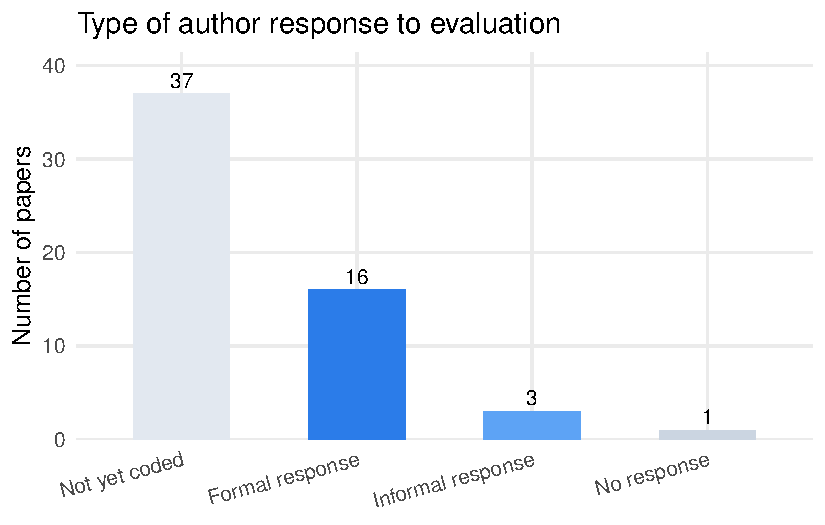
\includegraphics[keepaspectratio]{paper_response_analysis_files/figure-pdf/fig-response-bar-1.pdf}}

\end{figure}%

\subsection{Full Tabulation}\label{full-tabulation}

\begin{tcolorbox}[enhanced jigsaw, arc=.35mm, bottomrule=.15mm, bottomtitle=1mm, breakable, colback=white, colbacktitle=quarto-callout-note-color!10!white, colframe=quarto-callout-note-color-frame, coltitle=black, left=2mm, leftrule=.75mm, opacityback=0, opacitybacktitle=0.6, rightrule=.15mm, title=\textcolor{quarto-callout-note-color}{\faInfo}\hspace{0.5em}{All 57 tracked evaluations}, titlerule=0mm, toprule=.15mm, toptitle=1mm]

Click column headers to sort; use the search box to filter. Adjustment
status is color-coded: green = positive signal, orange =
minor/uncertain, grey = unlikely or not yet assessed.

\begin{table}[H]

\caption{\label{tbl-full}}

\begin{Shaded}
\begin{Highlighting}[]
\NormalTok{tbl }\OtherTok{\textless{}{-}}\NormalTok{ df }\SpecialCharTok{|\textgreater{}}
  \FunctionTok{mutate}\NormalTok{(}
    \AttributeTok{title\_linked =} \FunctionTok{if\_else}\NormalTok{(}
      \SpecialCharTok{!}\FunctionTok{is.na}\NormalTok{(pubpub\_link) }\SpecialCharTok{\&}\NormalTok{ pubpub\_link }\SpecialCharTok{!=} \StringTok{""}\NormalTok{,}
      \FunctionTok{paste0}\NormalTok{(}\StringTok{\textquotesingle{}\textless{}a href="\textquotesingle{}}\NormalTok{, pubpub\_link, }\StringTok{\textquotesingle{}" target="\_blank"\textgreater{}\textquotesingle{}}\NormalTok{,}
             \FunctionTok{str\_trunc}\NormalTok{(paper\_title, }\DecValTok{72}\NormalTok{), }\StringTok{\textquotesingle{}\textless{}/a\textgreater{}\textquotesingle{}}\NormalTok{),}
      \FunctionTok{str\_trunc}\NormalTok{(paper\_title, }\DecValTok{72}\NormalTok{)}
\NormalTok{    ),}
    \AttributeTok{authors\_short =} \FunctionTok{str\_trunc}\NormalTok{(authors, }\DecValTok{40}\NormalTok{),}
    \AttributeTok{nb\_icon =} \FunctionTok{if\_else}\NormalTok{(}
      \SpecialCharTok{!}\FunctionTok{is.na}\NormalTok{(nb\_link) }\SpecialCharTok{\&}\NormalTok{ nb\_link }\SpecialCharTok{!=} \StringTok{""}\NormalTok{,}
      \FunctionTok{paste0}\NormalTok{(}\StringTok{\textquotesingle{}\textless{}a href="\textquotesingle{}}\NormalTok{, nb\_link, }\StringTok{\textquotesingle{}" target="\_blank" title="NotebookLM"\textgreater{}\&\#128214;\textless{}/a\textgreater{}\textquotesingle{}}\NormalTok{),}
      \StringTok{""}
\NormalTok{    )}
\NormalTok{  ) }\SpecialCharTok{|\textgreater{}}
  \FunctionTok{select}\NormalTok{(}\AttributeTok{Paper =}\NormalTok{ title\_linked, }\AttributeTok{Authors =}\NormalTok{ authors\_short,}
         \AttributeTok{Area =}\NormalTok{ research\_area, }\AttributeTok{Response =}\NormalTok{ author\_response\_clean,}
         \AttributeTok{Adjustment =}\NormalTok{ adj\_status\_clean, }\StringTok{\textasciigrave{}}\AttributeTok{Pub.}\StringTok{\textasciigrave{}} \OtherTok{=}\NormalTok{ pub\_status, }\AttributeTok{NB =}\NormalTok{ nb\_icon)}

\NormalTok{adj\_bg }\OtherTok{\textless{}{-}} \FunctionTok{c}\NormalTok{(}
  \StringTok{"Evidence of updating"}        \OtherTok{=} \StringTok{"\#d4edda"}\NormalTok{,}
  \StringTok{"Stated intention to update"}  \OtherTok{=} \StringTok{"\#e8f5e9"}\NormalTok{,}
  \StringTok{"Mixed / minor updating"}      \OtherTok{=} \StringTok{"\#fff3e0"}\NormalTok{,}
  \StringTok{"Unlikely to update"}          \OtherTok{=} \StringTok{"\#fce4d4"}\NormalTok{,}
  \StringTok{"Not yet assessed"}            \OtherTok{=} \StringTok{"\#f8fafc"}
\NormalTok{)}

\FunctionTok{datatable}\NormalTok{(tbl, }\AttributeTok{escape =} \ConstantTok{FALSE}\NormalTok{, }\AttributeTok{rownames =} \ConstantTok{FALSE}\NormalTok{, }\AttributeTok{filter =} \StringTok{"top"}\NormalTok{,}
  \AttributeTok{options =} \FunctionTok{list}\NormalTok{(}
    \AttributeTok{pageLength =} \DecValTok{8}\NormalTok{, }\AttributeTok{autoWidth =} \ConstantTok{FALSE}\NormalTok{, }\AttributeTok{scrollX =} \ConstantTok{TRUE}\NormalTok{, }\AttributeTok{dom =} \StringTok{"lfrtip"}\NormalTok{,}
    \AttributeTok{columnDefs =} \FunctionTok{list}\NormalTok{(}
      \FunctionTok{list}\NormalTok{(}\AttributeTok{width =} \StringTok{"36\%"}\NormalTok{, }\AttributeTok{targets =} \DecValTok{0}\NormalTok{),}
      \FunctionTok{list}\NormalTok{(}\AttributeTok{width =} \StringTok{"18\%"}\NormalTok{, }\AttributeTok{targets =} \DecValTok{1}\NormalTok{),}
      \FunctionTok{list}\NormalTok{(}\AttributeTok{width =} \StringTok{"8\%"}\NormalTok{,  }\AttributeTok{targets =} \DecValTok{2}\NormalTok{),}
      \FunctionTok{list}\NormalTok{(}\AttributeTok{width =} \StringTok{"11\%"}\NormalTok{, }\AttributeTok{targets =} \DecValTok{3}\NormalTok{),}
      \FunctionTok{list}\NormalTok{(}\AttributeTok{width =} \StringTok{"16\%"}\NormalTok{, }\AttributeTok{targets =} \DecValTok{4}\NormalTok{),}
      \FunctionTok{list}\NormalTok{(}\AttributeTok{width =} \StringTok{"8\%"}\NormalTok{,  }\AttributeTok{targets =} \DecValTok{5}\NormalTok{),}
      \FunctionTok{list}\NormalTok{(}\AttributeTok{width =} \StringTok{"3\%"}\NormalTok{,  }\AttributeTok{targets =} \DecValTok{6}\NormalTok{)}
\NormalTok{    )}
\NormalTok{  ),}
  \AttributeTok{caption =} \StringTok{"All tracked Unjournal evaluations. NB = NotebookLM analysis link."}
\NormalTok{) }\SpecialCharTok{|\textgreater{}}
  \FunctionTok{formatStyle}\NormalTok{(}\StringTok{"Adjustment"}\NormalTok{,}
    \AttributeTok{backgroundColor =} \FunctionTok{styleEqual}\NormalTok{(}\FunctionTok{names}\NormalTok{(adj\_bg), }\FunctionTok{unname}\NormalTok{(adj\_bg)))}
\end{Highlighting}
\end{Shaded}

\end{table}%

\end{tcolorbox}




\end{document}
